% rubber: rules rules.ini
%
% PROJECT: <ETD> Electronic Thesis and Dissertation Initiative
%   TITLE: LaTeX report template for ETDs in LaTeX
%  AUTHOR: Neill Kipp, nkipp@vt.edu
%     URL: http://etd.vt.edu/latex/
% SAVE AS: etd.tex
% REVISED: September 6, 1997 [GMc 8/30/10]
% 

% Instructions: Remove the data from this document and replace it with your own,
% keeping the style and formatting information intact.  More instructions
% appear on the Web site listed above.

\documentclass[10pt]{report}

\usepackage{caption}
\DeclareCaptionType{copyrightbox}
% \ifCLASSINFOpdf   
%    \usepackage[pdftex]{graphicx}     
%    % declare the path(s) where your graphic files are       
%    \graphicspath{{../pdf/}{../jpeg/}{./image/}}    
%    % and their extensions so you won't have to specify these with    
%    % every instance of \includegraphics      
%    \DeclareGraphicsExtensions{.pdf,.jpeg,.png,.jpg}   
%  \else   
%    % or other class option (dvipsone, dvipdf, if not using dvips). graphicx     
%    % will default to the driver specified in the system graphics.cfg if no   % driver is specified.    
%    \usepackage[dvips]{graphicx}   
%    % declare the path(s) where your graphic files are     
%    \graphicspath{{../eps/}}    
%   % and their extensions so you won't have to specify these with   
%   % every instance of \includegraphics    
%   % \DeclareGraphicsExtensions{.eps}   
% \fi

\usepackage{subcaption}
\usepackage{url}
\usepackage{epstopdf}
\usepackage{multirow}
\usepackage{amsmath, amsfonts, amssymb}
\usepackage{graphicx}
\graphicspath{{./figures/}}
\usepackage{color}
%package for proper unicode rendering
\usepackage[utf8]{inputenc}
\usepackage{url}
\inputencoding{utf8}


\setlength{\textwidth}{6.5in}
\setlength{\textheight}{8.5in}
\setlength{\evensidemargin}{0in}
\setlength{\oddsidemargin}{0in}
\setlength{\topmargin}{0in}

\setlength{\parindent}{0pt}
\setlength{\parskip}{0.1in}

% Uncomment for double-spaced document.
% \renewcommand{\baselinestretch}{2}

% \usepackage{epsf}

\begin{document}

\thispagestyle{empty}
\pagenumbering{roman}

\newcommand{\then}{\Rightarrow}
\newcommand{\softor}{\operatornamewithlimits{\tilde{\vee}}}
\newcommand{\softand}{\operatornamewithlimits{\tilde{\wedge}}}
\newcommand{\softthen}{\operatornamewithlimits{\tilde{\then}}}
\newcommand{\softneg}{\operatornamewithlimits{\tilde{\neg}}}

\begin{center}

% TITLE
{\Large
    Forecasting Protests by Detecting Future Time Mentions in News and Social Media
}

\vfill

Sathappan Muthiah
\vfill

Dissertation submitted to the Faculty of the \\
Virginia Polytechnic Institute and State University \\
in partial fulfillment of the requirements for the degree of

\vfill

Master of Science\\
in \\
Computer Science and Applications

\vfill

Naren Rama, Chair \\
Chang Tien Lu \\
Graham E Katz \\

\vfill

June 26, 2014 \\
Arlington, Virginia

\vfill

Keywords: Textmining, Information Retrieval, Social Media
\\
Copyright 2014, Sathappan Muthiah

\end{center}

\pagebreak

\thispagestyle{empty}
\begin{center}

{\large Forecasting Protests by Detecting Future Time Mentions in News and Social Media
}

\vfill

Sathappan Muthiah

\vfill

(ABSTRACT)

\vfill

\end{center}

Civil unrest (protests, strikes, and ``occupy'' events) is a common occurrence in both democracies and authoritarian regimes. The study of civil unrest is a key topic for political scientists as it helps capture an important mechanism by which citizenry express themselves. In countries where civil unrest is lawful, qualitative analysis has revealed that more than 75\% of the protests are planned, organized, and/or announced in advance; therefore detecting future time mentions in relevant news and social media is a simple way to develop a protest forecasting system. We develop such a system in this paper, using a combination of key phrase learning to identify what to look for, probabilistic soft logic to reason about location occurrences in extracted results, and time normalization to resolve future tense mentions. We illustrate the application of our system to 10 countries in Latin America, viz. Argentina, Brazil, Chile, Colombia, Ecuador, El Salvador, Mexico, Paraguay, Uruguay, and Venezuela. Results demonstrate our successes in capturing significant societal unrest in these countries with an average lead time of 4.08 days. We also study the selective superiorities of news media versus social media (Twitter, Facebook) to identify relevant tradeoffs.
\vfill

% GRANT INFORMATION

% That this work received support from the Southeastern Universities
% Research Association (SURA) ``Monticello Library Project'' is purely
% coincidental.

\pagebreak

% Dedication and Acknowledgments are both optional
\chapter*{Dedication}

\vspace*{\fill}
\begin{center}
\Large\textit{To my wonderful Mom, Dad and Brothers}
\end{center}
\vspace{\fill}


\chapter*{Acknowledgments}
\vspace*{\fill}
\Large{First and foremost I would like to thank my advisor Dr.Naren Ramakrishnan. He was not only instrumental in kindling my interest in machine learning and data mining but is also my mentor in many ways. I also thank Dr Graham E Katz for his constant guidance and help with Software Integration.

I thank my Parents and Brothers for their great support without which i wouldnt have been able to complete.

I would like to thank my fellow graduate students Rupinder Paul Khandpur, Aravindan Mahendiran, Wei Wang, Fang jin, Prithwish Chakraborty, Parang Saraf, Saurav Ghosh and Michael Shuffet for their help and support throughout my graduate studies. 

I would like to thank Shahriar Hossain and Patrick Butler for their time and help on answering several of my queries.Also, i would like to thank Nathan Self for his help with visualizations and Jaime Arredondo for his help with building the keyphrase list.

I also like to thank all our collaborators at CACI inc., Andrew Doyle, Ilya Zavorin, Chris Ackerman, Jim Ford and Zunsik Lim for their help with Software Testing and Integration.

Finally I would also like to thank my roommates Rajesh Subbiah, Arvinth Chanthar Rathinama Saran Kumar and Chao Yang for making my stay at Blacksburg a memorable one
}
\vspace{\fill}



\tableofcontents
\pagebreak

\listoffigures
\pagebreak

\listoftables
\pagebreak

\pagenumbering{arabic}
\pagestyle{myheadings}

\chapter{Introduction}
\markright{Sathappan Muthiah \hfill Chapter 1. Introduction \hfill}
\label{intro}
\begin{figure}
    \centering
    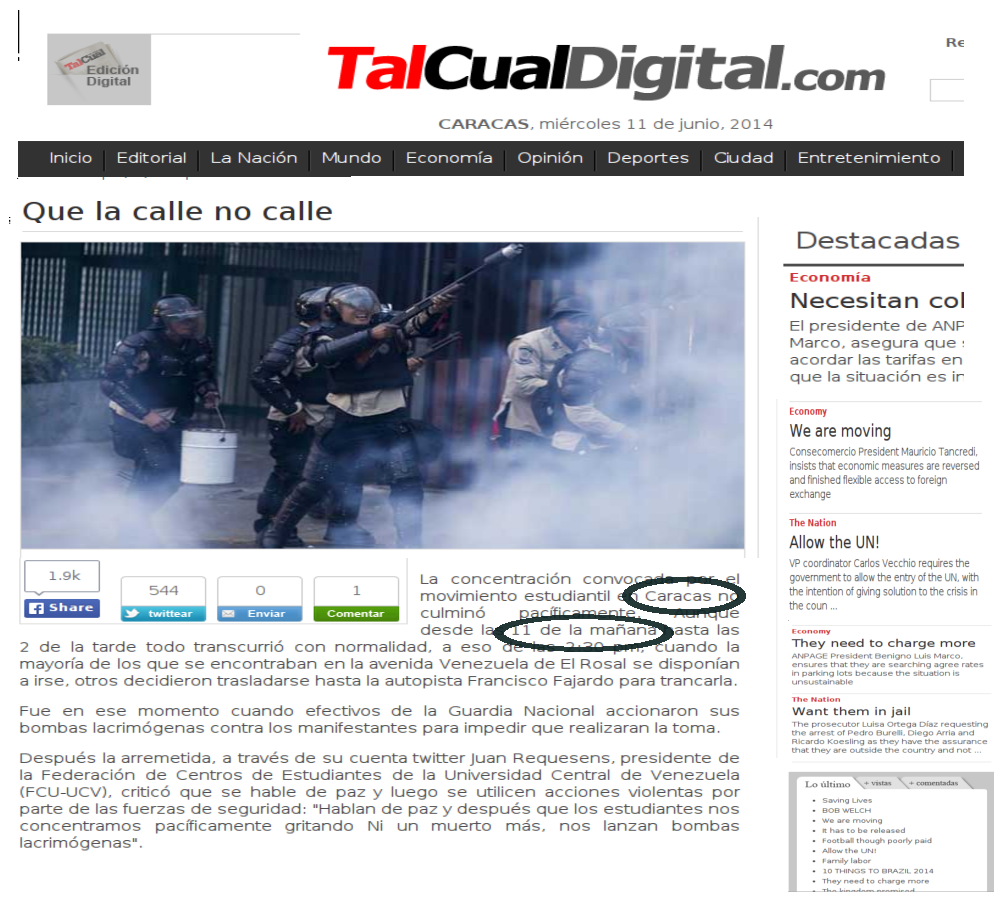
\includegraphics[scale=0.5]{pp_example}
    \caption{An example article describing plans for a future protest (Venezuela, June 11, 2014). The red and black circle show the identified location and date.}
    \label{pp_example}
\end{figure}
Civil unrest (protests, strikes, and ``occupy'' events) is a common happening in both democracies
and authoritarian regimes.
Although we typically associate civil unrest with disruptions and instability, for a social scientist
civil unrest reflects the democratic process by 
which citizenry communicate their views and preferences to those in authority. 
The advent of social
media has afforded citizenry new mechanisms for organization and mobilization, and online news sources
and social networking sites like Facebook and Twitter
can provide a window into civil unrest happenings in a particular country.

Our basic hypothesis is that
protests that are larger will be more disruptive and communicate support for its cause better than smaller protests. 
Mobilizing large numbers of people is more likely to occur if a protest is organized and the time and place announced in
advance. Because protest is costly and more likely to succeed if it is large, we should expect planned, rather than 
spontaneous, protests to be the norm. Indeed, in a sample of 288 events from our study selected for qualitative review of their antecedents
(more details later), for 225 we located communications regarding the upcoming occurrence of the event in media, and only 49 could be classified as 
spontaneous (we could not determine whether communications had or had not occurred in the remaining 14 cases).

We sought to develop
a computational protest forecasting system by
identifying and mining mentions of future planned events
in (news and social) media.  
Why is this problem difficult? Consider the example article shown in Fig.~\ref{pp_example},
covered in greater detail in Fig.~\ref{fig:psl_example}. Written in Spanish and published in Venezuela, it describes plans 
to protest on `Sunday' and mentions at least five different locations -- of which at least two are ambiguous and can either be in Colombia, Cuba or Venezuela. 
Significant reasoning is required to discern the correct protest location and to identify the intended date
from the vague reference of `Sunday.' Once the location and time of the future
protest are inferred, a suitably generated alert has applications to a wide range of 
governmental and civil activity, from the issuance of travel warnings
to rapid emergency response capabilities.  

Our detection approach 
combines shallow linguistic analysis to identify a corpus of relevant
documents (articles, tweets) which are then subject to targeted deep semantic analysis.
Despite its simplicity, we are able to
detect indicators of event planning with surprisingly high
accuracy. 
Our contributions are:
\begin{enumerate}
\item We present a protest forecasting system that couples three key technical ideas:
key phrase learning to identify what to look for, probabilistic soft logic to reason about location occurrences in extracted results, and 
date normalization to resolve future tense mentions. We demonstrate how the integration of these ideas achieves objectives in precision,
recall, and quality (accuracy).
\item We illustrate the application of our system to 10 countries in Latin America, viz. Argentina, Brazil, Chile, Colombia, Ecuador, El Salvador, Mexico, Paraguay, Uruguay, and Venezuela. 
We conduct ablation studies to identify the 
relative contributions of news media (news + blogs) versus social media (Twitter, Facebook) to identify future happenings of
civil unrest. Through these studies we illustrate the selective superiorities of different sources for specific countries.
\item Unlike many studies of retrospective forecasting of protests,
we assess the lead time from when the forecast is made to
the actual event date, to assess the forecasting prowess of our approach. 
Our results demonstrate that we are able to 
capture significant societal unrest in the above countries with an average lead time of 4.08 days. This illustrates that the
approach here can be used in a practical protest forecasting system.
\end{enumerate}


%%%%%%%%%%%%%%%%%
%
% Include an EPS figure with this command:
%   \epsffile{filename.eps}
%

%%%%%%%%%%%%%%%%
%
% Do tables like this:
\chapter{Related Work}
\markright{Sathappan Muthiah \hfill Chapter 2. Related Work \hfill}
Five categories of related work 
%-- \emph{Event Detection, Temporal Information Extraction, Future Retrieval, Extraction of Planned Events and Event Forecasting} -- 
are briefly discussed here.
\begin{table*}
    \centering
    \caption{Comparison of our approach against other future retrieval techniques.}
    \begin{tabular}{l p{1.6cm} p{2cm} p{2cm} p{1.8cm} p{3cm}}%{|*{17}{c|}}
        \hline
        & Relative date resolution & Ingest multiple sources? & {\bf Reasoning about location} & {\bf Learning word/phrase filters} \\
        \hline
        `Future' Search Engines~\cite{Kawai:2010:CSE, Jatowt:2011:ECE,baeza2005searching}&\checkmark & & \\
        Time-to-Event Recognition~\cite{tops2013predicting, bosch2013estm}&\checkmark & & \\
        Planned Protest Detection~\cite{xu2014civil,compton2013detecting} & &\checkmark & &\\ 
        {\bf This thesis} &\checkmark &\checkmark &\checkmark&\checkmark\\  \hline
\end{tabular}
\label{comp-table}
\end{table*}
\section{Event detection via text extractions}
\vspace{-.8em}
Event Detection is an extensively studied topic in the literature. Document clustering techniques are used 
in~\cite{Allan:2002:TDT, Yang:1998:SRO, Gabrilovich:2004:NPP} to identify events retrospectively or as the stories arrive.
Works like~\cite{Banko07openinformation, Chambers:2011:TIE, riloff2003learning} focus on
extraction patterns (templates) to extract information from text. Ritter et al.~\cite{Ritter:2012} show that
it is possible to accurately extract a calendar of significant events from Twitter by training a tagger for recognizing event phrases.
\iffalse 
Sankaranarayanan et al.~\cite{Sankaranarayanan:2009:TNT} captures tweet clusters of interest to identify late breaking News from twitter 
\fi
Highly specialized applications
also exist; e.g., Sakaki et al.~\cite{Sakaki:2010:EST} mine tweets to enable prompt detection of occurences of earthquakes.

\section{Temporal information extraction} 
\vspace{-.8em}
Temporal Information Extraction is another well studied topic.
The TempEval challenge~\cite{tempeval} led to a significant amount of
algorithmic development for temporal NLP.
For instance, a specification language
for temporal and event expressions in natural language text is described in~\cite{timeml}.
Refs.~\cite{LlorensDGS12} and~\cite{tempex} provide methods to resolve temporal expressions in text (our own
work here uses the TIMEN package~\cite{LlorensDGS12}).
\vspace{-.8em}

\section{Event forecasting}
\vspace{-.8em}
Event forecasting is a burgeoning area. 
Radinsky and Horvitz~\cite{Radinsky:2013:MWP} find event sequences from a corpora and then use these sequences to determine if 
an event of interest (e.g., a disease outbreak, or a riot)
will occur sometime in the future. This work predicts only if a potential event will happen given a historical event sequence
but does not geolocate the event to a city-level resolution, as we do here.
Kallus~\cite{nathankallus} makes use of event data from 
RecordedFuture~\cite{recordedFuture} to determine if a  significant protest event will occur in 
the subsequent three days and casts this as a classification problem.
This work only focuses on prediction of significant events (suitably defined) and
the forecast is limited to the next three days. Ramakrishnan et al.~\cite{emberskdd} describe the EMBERS
system for forecasting civil unrest using open source indicators but this work is primarily focused on shallow mining of
a broad set of data sourceas in contrast to the focused analysis of planned protest announcements that we study here.
\vspace{-.8em}

\section{Future Retrieval}
\vspace{-.8em}
Finally, Future Retrieval, an emerging research topic, is another area of research most closely related to our work.
Baeza-Yates~\cite{baeza2005searching} providing one of the earliest discussions
of this topic; here future temporal information in text is found and used to retrieve content from search queries that 
combine both text and time with a simple ranking scheme. Kawai et al.~\cite{Kawai:2010:CSE} present a search engine (ChronoSeeker) for searching 
future and past events.
They make use of an SVM classifier to disambiguate between the various temporal expressions in a document.
Dias et al.~\cite{dias2011future} classify web snippets into three classes depending on if a future date can/cannot be predicted 
from the snippet or if it is a rumor.
%{\bf Extraction of planned or future mentions of events from social media} is a very popular topic in social media
%analytics.
RecordedFuture~\cite{recordedFuture}, introduced earlier, conducts
real-time analysis of news and tweets to identify mentions of events along with associated times. Anectodally it 
is estimated that approximately (only) 5--7\% of events extracted 
by RecordedFuture are about the future.
Tops et al.~\cite{tops2013predicting} aim to classify a tweet talking about an event into discrete time segments and thereby predict the 
`time to event'.
Bosch et al.~\cite{bosch2013estm} use regression techniques to identify the time to an event referred to by a tweet.
Jatowt et al.~\cite{Jatowt:2011:ECE} provide a collective image of the future associated with an entity summarizing all future related information available.
Becker et al.~\cite{Becker:2012:ICP} try to identify more content about known planned events (e.g., a concert) across social media. This work
for instance assumes that we know the event beforehand and aims to identify relevant details of the event.

%\cite{baeza2005searching},\cite{dias2011future},\cite{tops2013predicting},\cite{Jatowt:2011:ECE},\cite{Kawai:2010:CSE} talk about future retrieval or extraction of mentions of Future events.
In particular, two publications---Compton et al. ~\cite{compton2013detecting} and Xu et al.~\cite{xu2014civil}---align very closely to our own work as their emphasis is on protest forecasting.
Both works are aimed at forecasting protests
but emphasize different data sources and different methodologies. For instance, the work in~\cite{compton2013detecting} filters the Twitter stream for
keywords of interest and searches for future date mentions in only absolute terms, i.e., explicit mentions of a month name and a number (date)
less than 31. 
Such an approach will not be capable of extracting the more
common way in which future dates are referenced, e.g., phrases like
``tomorrow,'' ``next tuesday.'' 
%Any location mentioned in the tweet text is used as the event location. If there are no location mentions then the location is determined based on~\cite{hrlgeocoder}. 
The work in~\cite{xu2014civil} by the same group of authors uses the Tumblr feed with a smaller set of keywords but
again is restricted to the use of absolute time identifiers.

In surveying the state-of-the-art, we arrived at desiderata for a planned protest forecasting system. As shown in Table~\ref{comp-table},
we desire a system that is capable of: i) ingesting a broad range of data sources from both popular news and social media,
ii) learning relevant phrases for tracking protests, 
iii) handling relative mentions of dates, and
iv) providing a rich representational and reasoning basis for location. 
As Table~\ref{comp-table} summarizes, current systems provide only partial solutions and the proposed
approach addresses all four desired criteria.

\section{Geocoding}
A News report, blog posting or a tweet can have multiple locations associated with it. It is necessary to disambiguate each of these locations and try to identify what they refer to -- whether they refer to the location from where the document is written, users home location or the geo-focus of the content etc.

Identifying the different geographical locations associated with a tweet/news document is of great interest to the researchers recently.
David et al.~\cite{hrlgeocoder}, Lindamood et al.~\cite{inferringSN} and Backstrom et al.~\cite{findMe} talk about using the network information based on social relationships to infer an users location.These approaches infer locations by spatially propagating location assignments through the social network, using a samll number of known users/locations. Such approaches are mostly based on the assumption that people we interact with on a daily basis always live near us.

Amitay et al.~\cite{amitay2004web}, Fink et al.~\cite{geoBlogs},Cheng et al.~\cite{youAreTweet}, etc., use content based approaches to determine a documents location. Yin et al.~\cite{geoTopic} introduces a topic modelling approach called Latent Geographical Topic Analysis, that combines location and text to identify topics specific to a geographical area. These topics can then be used as important cures to group different geographical regions and also to identify the location of new users based on the content they publish.

Some work has also been done where both knowledge from the content and network are used to infer the location. In ~\cite{geoUserprofiling} Li et al.  builds a unified discriminative influence model to  combine both socail network information and the user-centric information available from his/her tweeting history using a probabilistic framework. Li et al., in yet another work ~\cite{geoMLP}, try to capture the location profile of an user from their followers network and tweet history and also profile the users location for each avaliable relationship in the network.

For our purpose, we try to distinguish between an users home location and the tweets content location.  Thus, we mainly make use of content based approaches for identifying the geographical focus of a document. The approach used is described in detail in section~\ref{sec:geocoding}.


\chapter{Preliminaries}
\markright{Sathappan Muthiah \hfill Chapter 3. Preliminaries  \hfill}
Our emphasis in this work is on Latin America.
Protest is an important topic of study in this
region, as many countries here are democracies struggling to consolidate themselves.
The combination of weak channels of communication between citizen and government, and a citizenry that still 
has not grasped the desirability of elections as the means to affect politics means that public protest 
will be an especially attractive option. To illustrate the power of protest in Latin America we need 
only recall that between 1985 and 2011, 17 presidents resigned or were impeached under pressure from 
demonstrations, usually violent, in the streets. Protests have also resulted 
in the rollback of price increases for public services, such as during the `Brazilian Spring' of June 2013.
\begin{figure}
    \centering
    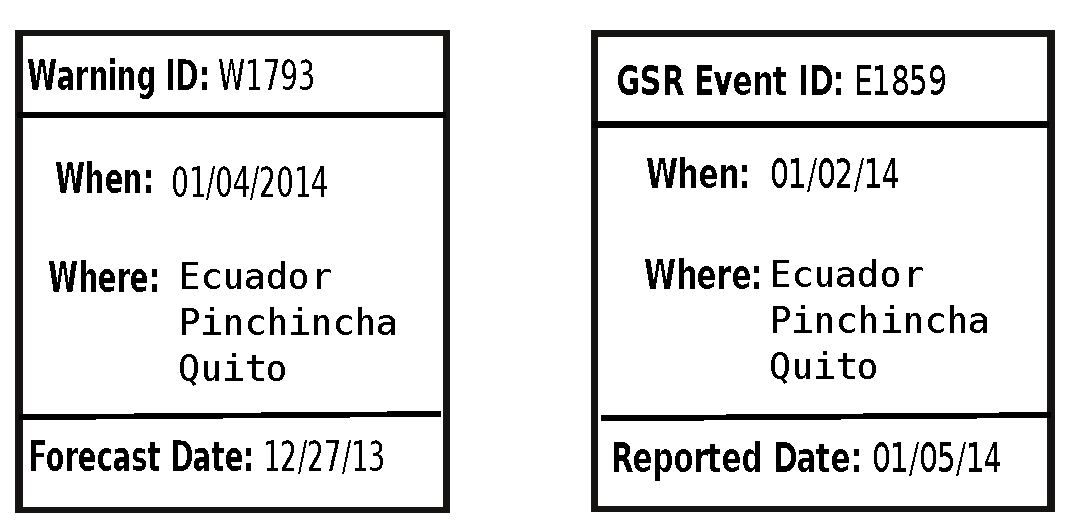
\includegraphics[scale=0.5]{alertstructure}
    \caption{An example warning (left) and GSR event (right).}
    \label{fig:alertstructure}
\end{figure}
Our goal is to identify calls for protests, strikes, or civil disobedience movements from news, blogs, Tweets, and Facebook
pages, with a view toward predicting the {\bf when} (date of the event) and {\bf where}, i.e.,
event location, up to city-level resolution, e.g., 
the city of {\it Tegucigalpa} in the state of {\it Francisco Morazan} in the country of {\it Honduras}).
\iffalse
In addition we seek to forecast the `why' and `who' of the protest.
The {\bf why} (or event type)
captures the main objective or reason for a civil unrest event,
and is meant to come from 7 broad classes (e.g., `Employment \& Wages',
`Housing', `Energy \& Resources' etc.) each of which is further categorized into
whether the event is forecast to be violent or not.
Finally, the {\bf who} (or population)
denotes common categories of human populations
used in event coding~\cite{philschrodt}
such as
Business, Ethnic, Legal (e.g. judges or lawyers), Education (e.g. teachers or students or parents of students), Religious (e.g. clergy), Medical (e.g., doctors or nurses), Media, Labor, Refugees/Displaced, Agricultural (e.g. farmers,
or just General Population. 
\fi
We refer to our forecasts as alerts or warnings (see Fig.~\ref{fig:alertstructure} (left)).
In looking at the structure of the alert, it is important to distinguish between the forecast date (when the forecast is made)
and the predicted event date (i.e., the {\bf when} of the event).


%Concomitant with the definitions in the above section, a GSR event contains
%again the where/why/when/\hskip0ex who of a protest that has actually occurred and
%a {\it reported date} (the date a newspaper reports the protest as
%having happened).
%See Fig.~\ref{fig:alertstructure} (right).
%The GSR is organized by an
%independent third party (MITRE) and the authors of this study do not
%have any participation in this activity. 
\section{Evaluation Metrics -- Quality score}
To evaluate our alerts we have access to a database of protests organized by a third party (source and reference
not provided due to double blind reviewing considerations, but will be added later). We refer to this database as the
GSR (for Gold Standard Report). Human analysts scan newspapers of record in the countries of interest and catalog
protests. The structure of a GSR event (see Fig.~\ref{fig:alertstructure} (right)) is similar to that of an alert with
the only difference being that an event record captures both the reported date (i.e., the date of newspaper publication)
and the event date (i.e., when the newspaper article reports the protest as having happened).
The GSR is available from Nov 2012 
and is used in this thesis primarily to 
help evaluate the performance of our system. A manual examination of GSR (as mentioned in Section~\ref{intro}) revealed
that over 75\% of the protests were organized and had clear triggering circumstances with political entrepreneurs leading the
charge to protest.

\subsection{Lead Time vs Accuracy of Forecast Date}
It is important to understand which alerts {\it can} be matched to specific events.
Note that there are four dates in an (alert,event) combination (see Fig.~\ref{fig:timeline}):
\begin{enumerate}
\item The date the forecast is made ({\it forecast date})
\item The date the event is predicted to happen ({\it predicted event date})
\item The date the event actually happens ({\it event date})
\item The date the event is reported in a GSR source ({\it reported date})
\end{enumerate}

\begin{figure}[t]
\centering
\includegraphics[width=0.40\textwidth]{figures/timeline}
\caption[Timeline depicting lead-time vs date accuracy]{Alert sent at time $t1$ predicting an event at time $t3$
can be matched to a GSR event that happened at time $t2$ and reported
at time $t4$ if $t1 < t4$.}
\label{fig:timeline}
\end{figure}

For an event to be qualified as having been predicted by a warning,
{\it forecast date} $<$ {\it reported date}
(recall that time is measured in
granularities of days).
The {\it lead time} is given as
$(\textit{reported date} - \textit{forecast date})$, i.e., the number
of days by which we `beat the news.'
In constrast, the difference between
{\it predicted event date} and {\it event date}, i.e.,
$|\textit{event date} - \textit{predicted event date}|$.
is one of {\it quality} or accuracy.
Ideally we require {\it lead time} to be as high as possible and
$|\textit{event date} - \textit{predicted event date}|$ to be as low
as possible.

\subsection{Other Quality Aspects}
Forecasting the event date accurately is only one aspect of quality.
Recall that alerts also forecast the location. A scoring formula is also defined for the location quality and 
overall quality score is defined as a sum over both the date and location scores.
$$\textrm{Quality score } (QS) = (DS + LS)*2$$
where DS and LS denote the date score and location score, respectively.
Each of these scores is in turn defined next:
$$DS = 1 - \min(|\textit{event date} - \textit{predicted event date}|,7)/7$$
If the date of the event listed in the warning is the same as the
actual date of the event, then $DS$ is 1. On the other hand, if these dates
are farther than 7 days apart, then $DS$ is 0.

Location score (LS) can be defined in many ways. Because location is
defined in terms of triples of (country, state, city), one approach is
to use a tiered formula. Comparing a GSR event with a warning, we can
obtain a score triple of $(l_1, l_2, l_3)$ where $l_1$ is the
country-level score, $l_2$ is the state-level score, and $l_3$ is the
city-level score. Each of these scores have a value of $0$ if they
do not match and $1$ is they match. Then the match between submitted
warning location and the GSR location is given by:
$$LS = {1 \over 3} l_1 + {1 \over 3} l_1 l_2 + {1 \over 3} l_1 l_2 l_3$$
\noindent
An alternative way to define location score is as:
$$LS = (1 - \min(\textrm{dist},300)/300)$$
where $\textrm{dist}$ denotes the distance (in km) between the city predicted and
the GSR city. All city location names are standardized to the World Gazeteer which provides
latitude and longitude values, thus facilitating the computation of distance.
We use the physical distance based criteria for our purposes.

\subsection{Inclusion Criteria}
Thus far we have demonstrated, given a warning-event pair, how we can
score their fitness. Inclusion criteria define which W-E pairs {\it can}
even be considered for scoring. We have already mentioned one inclusion
criterion, viz. that lead time must be $> 0$. The full list of inclusion
criteria we will consider are:
\begin{enumerate}
\item Lead time $> 0$
\item Both warning and event are for the same country.
\item The {\it predicted event date} and {\it event date} must be
within 7 days of each other.
\end{enumerate}
A fourth, optional (and stringent), criterion we will use is:
%\narenc{Patrick, fix the below enumerate so that it starts at 4.} done
\begin{enumerate}
  \setcounter{enumi}{3}
  \item Both predicted location and event location must be within 300km of
each other.
\end{enumerate}
It is important to distinguish the inclusion criteria from the scoring
criteria. Inclusion criteria define which W-E pairs are allowable.
Scoring criteria determine, from these allowable W-E pairs, what their
score will be.

\subsection{Matching Alerts to Events}
Thus far we have assumed that we matching an alert to a GSR event. In
practice, the problem is we are given a set of issued alerts  and a set
of GSR events and we must determine the quality of the match: which
alert would correspond to which event? One strategy is to construct
a bipartite graph between the set of alerts and the set of events,
where allowable edges are those that satisfy the inclusion criteria, and
where weights on these allowable edges denote their quality scores.
We then construct
a maximum weighted bipartite matching, e.g., see
Fig.~\ref{fig:matching} (middle). Such matchings are conducted on a monthly basis
with a lookback period to bring in unmatched warnings from the previous month.

\begin{figure}[t]
\centering
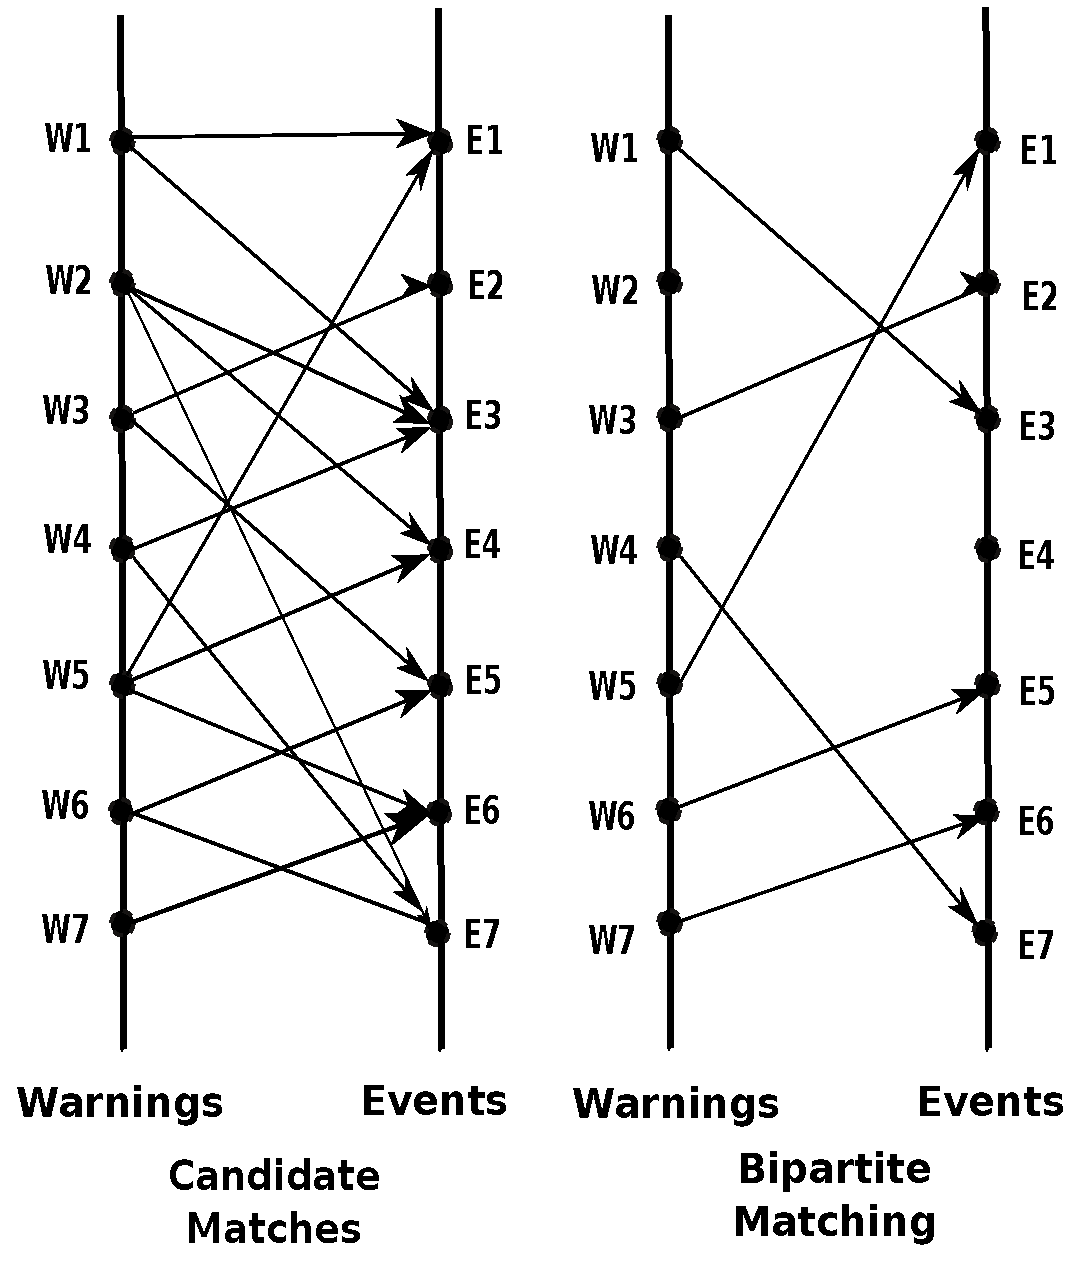
\includegraphics[width=0.50\textwidth]{figures/matching.pdf}
\caption[An example of the bipartite matching used for evaluation]{Given a set of candidate warning-event matches (left), we evaluate the
performance of EMBERS using either a regular bipartite matching (middle) or
by constructing a non-crossing matching (right).}
\label{fig:matching}
\end{figure}


%\subsection{Lead Time vs Accuracy of Forecast Date}
%Before we explain how alerts are matched to events, it is important to
%first understand which alerts {\it can} be matched to specific events.
%Note that there are four dates in an (alert,event) combination (see Fig.~\ref{fig:timeline}):
%\begin{enumerate}
%\item The date the forecast is made ({\it forecast date})
%\item The date the event is predicted to happen ({\it predicted event date})
%\item The date the event actually happens ({\it event date})
%\item The date the event is reported in a GSR source ({\it reported date})
%\end{enumerate}

\iffalse
\subsection{Quality Score}
The Quality score is defined as $$QS = (LS + DS)*2$$ where LS and DS denote location score and date score respectively. The location score is defined based on the kilometre distance between the predicted location and actual location. An alert can be matched to an event, if and only if it is within a 300km radius of the event location. The location score for an alert $Y$ with respect to an event $X$ is defined as $$LS=1 - min(dist(X,Y), 300) / 300 $$
The date score is defined similarly as $$DS = 1 - min( (X-Y), MAXINTERVAL)/MAXINTERVAL$$ where MAXINTERVAL  can be anything. For our experiments, a MAXINTERVAL of 7 days is used. Again a matching cannot occur if $DS=0$
\fi


\chapter{Probabilistic Soft Logic}
\markright{Sathappan Muthiah \hfill Chapter 4. Probabilistic Soft Logic \hfill}
%!TEX root = ../plannedprotest.tex

%\iffalse
%To extract the protest location from news articles, we use \emph{probabilistic soft logic} (PSL) \cite{broecheler:uai10} to build a model that performs robust, probabilistic inference given noisy signals. PSL takes a set of weighted, logic-like rules and converts them into a continuous probability distribution over the unknown truth values of logical facts. These truth values in PSL are relaxed into the $[0,1]$ interval. We use this mechanism to build a model that infers the semantic location of an article by weighing evidence coming from the Basis entity extractions and information in the World Gazatteer. 
%
%The primary rules in the model encode the effect that Basis-extracted location strings that match to gazatteer aliases are indicators of the article's location, whether they be country, state, or city aliases. Each of these implications is conjuncted with an prior for ambiguous, overloaded aliases that is proportional to the population of the gazetteer location. For example, if the string ``Los Angeles'' appears in the article, it could refer to either Los Angeles, California, or Los \'{A}ngeles in Argentina or Chile. Given no other information, our model would infer a higher truth value for the article referring to Los Angeles, California, because it has a much higher population than the other options. 
%
%The secondary rules, which are given half the weight of the primary rules, perform the same mapping of extracted strings to gazetteer aliases, but for extracted persons and organizations. Strings describing persons and organizations often include location clues (e.g., ``mayor of Buenos Aires''), but intuition suggests the correlation between the article's location and these clues may be lower than with location strings. 
%
%Finally, the model includes rules and constraints to require consistency between the different levels of geolocation, making the model place higher probability on states with its city contained in its state, which is contained in its country. As a post-processing step, we enforce this consistency explicitly by using the inferred city and its enclosing state and country, but adding these rules into the model makes the probabilistic inference prefer consistent predictions, enabling it to combine evidence at all levels.
%\fi

In this section, we briefly describe probabilistic soft logic (PSL)~\cite{kimmig2012short}, a key
component of our geocoding strategy described later.
PSL is a framework for collective probabilistic reasoning on relational domains.
PSL models have been developed in various domains, including collective classification~\cite{broecheler2010computing}, 
ontology alignment~\cite{brocheler2012probabilistic}, personalized medicine~\cite{bach2010decision}, 
opinion diffusion~\cite{bach2012scaling} , trust in social networks~\cite{huang2012probabilistic}, and graph 
summarization~\cite{memory2012graph}.
PSL represents the domain of interest as logical atoms.
It uses first order logic rules to capture the dependency structure of the domain, based on which it builds a joint probabilistic model over all atoms.
Instead of hard truth values of $0$ (false) and $1$ (true), PSL uses soft truth values relaxing the truth vlaues to the interval $[0,1]$.
The logical connectives are adapted accordingly.
This makes it easy to incorporate similarity or distance functions.

User defined \emph{predicates} are used to encode the relationships and attributes and \emph{rules} capture the  dependencies and constraints.
Each rule's antecedent is a conjunction of atoms and its consequent is a dis-junction. 
The rules can also labeled with non negative weights which are used during the inference process.
The set of predicates and weighted rules thus make up a PSL program where known truth values of ground atoms derived from observed data and unknown truth values for the remaining atoms are learned using the PSL inference.

Given a set of atoms 
$\ell = \{\ell_1,\ldots,\ell_n\}$,
an interpretation defined as 
$I : \ell \rightarrow [0,1]^n$
is a mapping from atoms to soft truth values.
PSL defines a probability distribution over all such interpretaions such that those that satisfy more ground rules are more probable.
\emph{Lukasiewicz t-norm} and its corresponding co-norm are used for defining relaxations of the logical AND and OR respectively to determine the degree to which a ground rule is satisfied.
Given an interpretation $\mathit{I}$, PSL defines the formulas for the relaxation of the logical conjunction ($\wedge$), disjunction ($\vee$), and negation ($\neg$) as follows:

\begin{align*}
\ell_1 \softand \ell_2 &= \max\{0, I(\ell_1) + I(\ell_2) - 1\},\\
\ell_1 \softor \ell_2 &= \min\{I(\ell_1) + I(\ell_2), 1\},\\
\softneg l_1 &= 1 - I(\ell_1),
\end{align*}  

The interpretation $\mathit{I}$ determines whether the rules is satisfied, if not, the \emph{distance to satisfaction}.
A rule $\mathit{r} \equiv \mathit{r_{body}} \rightarrow \mathit{r_{head}} $  is satisfied if and only if the truth value of head is at least that of the body. The rule's distance to satisfaction measures the degree to which this condition is violated.
 \newline
\begin{center} 
 $\mathit{d_r}(\mathit{I}) =$ max\{0,$\mathit{I(r_{body})} - \mathit{I(r_{head})}$\}
 \end{center}

PSL then induces a probability distribution over possible interpretations $\mathit{I}$ over the given set of ground atoms $\mathit{l} $ in the domain. 
If $\mathit{R}$ is the set of all ground rules that are instances of a rule from the system and uses only the atoms in  $\mathit{I}$ then,
the probability density function $\mathit{f}$ over $\mathit{I}$ is defined as
\begin{equation}
\label{eq:contimn1}
    f (I) = \frac{1}{Z} \text{exp}[-\sum_{r\in R} \lambda_r (d_r(I))^p]
\end{equation}
\begin{equation}
\label{eq:contimn2}
	Z = \int_{I} \text{exp} [ -\sum_{r\in R} \lambda_r (d_r(I))^p ]
\end{equation}
where~$\lambda_r$ is the weight of the rule~$r$, $Z$ is the continuous version of the normalization constant used in discrete Markov random fields, and ~$p \in \{1, 2\}$ provides a choice between two different loss functions, linear and quadratic.
The values of the atoms can be further restricted by providing linear equality and inequality constraints allowing one to encode functional constraints from the domain. 

PSL provides for two kinds of inferences:
(a) most probable explanation and (b) calculation of the marginal distributions. 
In the MPE inference given a partial interpretation with grounded atoms based on observed evidence, the PSL program infers the truth values for the unobserved atoms satisfying the most likely interpretation. 
In the second setting, given ground truth data for all atoms we can learn the weights for the rules in our PSL program.

\label{section:PSL}

\chapter{Approach}
\markright{Sathappan Muthiah \hfill Chapter 5. Approach \hfill}
\begin{figure*}
\centering
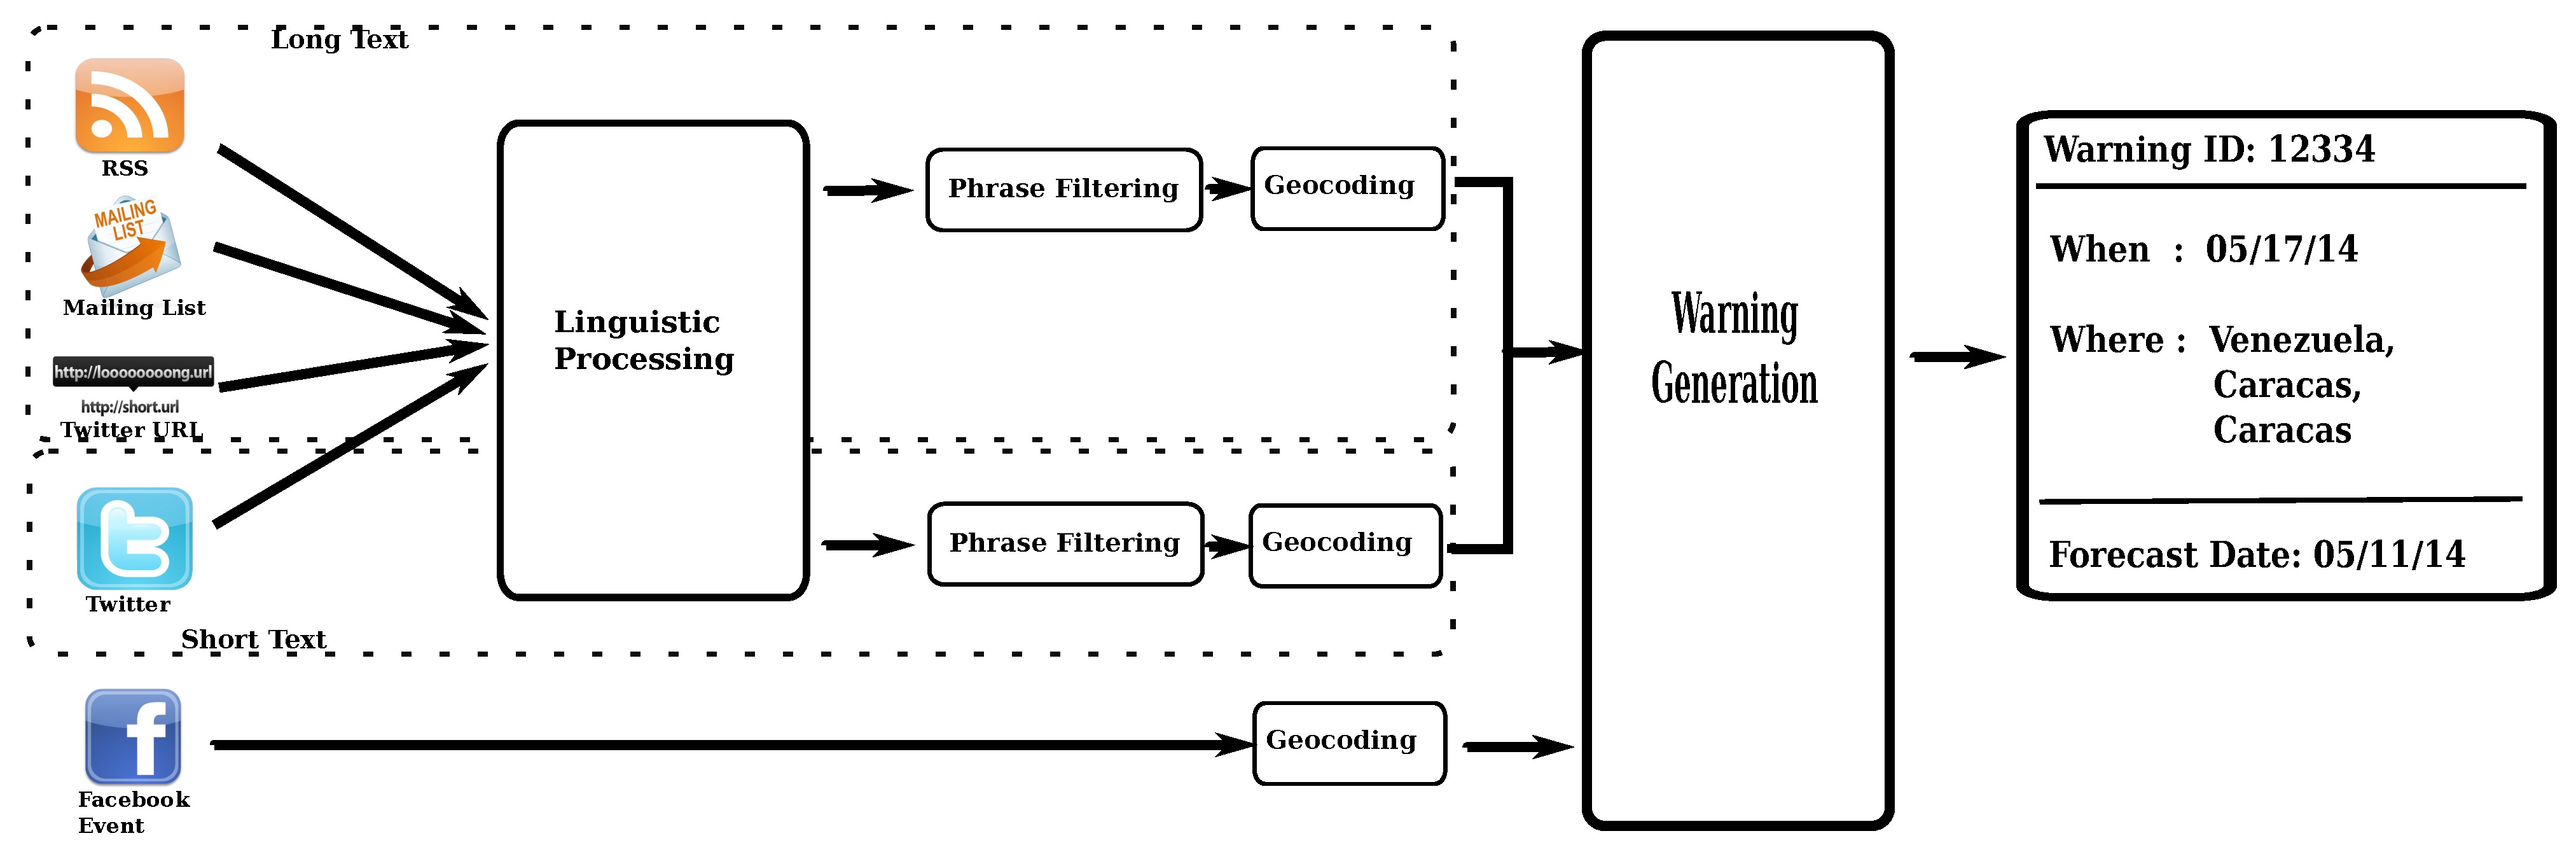
\includegraphics[width=\textwidth]{pipeline}
\caption{Schematic of the planned protest detector that ingests five
different types of data sources.}
\label{flowchart}
\end{figure*}
The general approach we adopt is to identify open-source documents
that appear to indicate civil unrest event planning, extract
relevant information from identified documents and use that as the
basis for a structured warning about the planned event (see Fig.~\ref{flowchart}).
We ingest a
wide array of textual documents, including RSS feeds (news and blogs),
mailing lists, URLs referenced in tweets, the contents of the tweets themselves,
and Facebook event pages.
All harvested documents are subjected to linguistic analysis; candidate
documents are identified using a list of (learnt) phrases associated with
protest event planning; date and location information is extracted from the
text and reasoned about to generate a warning. Location information is standardized
to conform to a standard (in our case, we use the World Gazeteer).
Each of these processing
steps (see Fig.~\ref{flowchart}) is outlined next.

\section{Linguistic Preprocessing}
All textual input (e.g., tweets, news articles, blog postings) is
subjected to shallow linguistic processing prior to analysis.  This
involves identifying the language of the document, distinguishing
the words (tokenization), normalizing words for inflection
(lemmatization), and identifying expressions referring to people,
places, dates and other entities and classifying them (named entity extraction). 
Since our region of interest is Latin America, the collection of text
harvested is inherently multilingual, with Spanish, Portugese, and English as
the dominating languages;
we use Basis Technology's Rosette Linguistics Platform (RLP) suite of multilingual commercial tools (\url{http://www.basistech.com/text-analytics/rosette/}) for this stage.
The output of linguistic preprocessing serves as input to subsequent deeper analysis in which 
date expressions are normalized and the geographic focus of the text identified.

Date processing is particularly crucial to the identification of
future oriented statements. We use the TIMEN~\cite{LlorensDGS12} date
normalization package to normalize and deindex expressions referring
to days in English, Spanish and Portuguese. This system makes use of
meta-data such as the day of publication, and other information about
the linguistic context of the date expression to determine for each
date expression, what day (or week, month or year) it refers to.  For
example in a tweet produced on June 10, 2014, the occurrence of the
term {\em Friday} used in a future-tense sentence {\em We'll get
  together on Friday} will be interpreted as June 13, 2014.  Each
expression identified as a date by the RLP preprocessor is normalized
in this way.

\section{Phrase filtering}
In order to identify relevant documents, input documents are filtered on a set of key phrases, i.e.,
the text of the document is searched for the presence of one or
more key phrases in a list of phrases which are indicative of an article's focus being
a planned civil unrest event.  
The list of key phrases indicating civil unrest planning was obtained
in a semi-automatic manner, as detailed in Section \ref{sec:phraselearning}.
Articles which do match are processed further, those that do not are ignored.

\subsection{Phrase matching}
Our key phrase matching is highly general and linguistically
sophisticated.  The phrases in our list are general rules for
matching, rather than literal string sequences. Typically a phrase
specification comprises: two or more word lemmas, a language
specification, and a separation threshold. This indicates that words---potentially inflected forms---in 
a given sequence potentially separated by one or more other words, should be taken to be a
match. We determined that this kind of
multi-word key phrases was more accurate than simple keywords for
extracting events of interest from the data stream.

The presence of a keyphrase is checked by searching for the presence of
individual lemmas of the keyphrase within the same sentence separated
by at most a number of words that is fewer than the separation threshold.  
This method allows for linguistically sophisticated and flexible matching, so, for example,
the keyphrase {\bf [{\em plan protest}, 4, English]} would match the sentence
{\em The students are planning a couple big protests tomorrow} in an input document.

\subsection{Phrase list development}
\label{sec:phraselearning}
The set of key phrases was tailored (slightly) to the genre of the
input. In particular different phrases were used to identify relevant
news articles and blogs from those used to filter Tweets.  The lists
themselves were generated semi-automatically.

Initially, a few seed phrases were obtained manually
with the help of subject matter experts.
An analysis of news reports for planned protests in the print media helped create a
minimum set of words to use in the query.  We choose four nouns from
the basic query that is used predominantly to indicate a civil unrest
in the print media - {\em demonstration, march, protest} and
{\it strike}. We translated them into Spanish and Portuguese, including
synonyms.  We then combined these with future-oriented verbs, e.g., {\em to organize}, {\em to prepare}, {\em to
plan}, and {\em to announce}. For twitter, shorter phrases were identified, and these had
a more direct call for action, e.g., {\em marchar}, {\em manhã de mobilização}, {\em
  vamos protestar}, {\em huelga}.

To generalize this set of phrases, the phrases were then parsed
using a dependency parser~\cite{freeling} and the grammatical
relationship between the core nominal focus word (e.g., {\em protest}, 
{\em manifestación}, {\em huelga}) and any accompanying
word (e.g., {\em plan}, {\em call}, {\em anunciar}) was
extracted. These grammatical relations were used as extraction
patterns as in~\cite{riloff2003learning} to learn more phrases from a
corpora of sentences extracted from the data stream of interest
(either news/blogs or tweets). This corpus consists of sentences that
contained any one of the nominal focus words and also had mentions of
a future date. The separation threshold for a phrase was also
learned, being set to the average number of words separating
the nominal focus and the accompanying word.

The set of learned phrases is then reviewed by a subject matter expert for quality contraol.  
Using this approach, we learned 112 phrases for news articles and blogs and 156 for tweets.  
This phrase learning process is illustrated in Fig.~\ref{fig:phraselearning}.

\begin{figure}
\centering
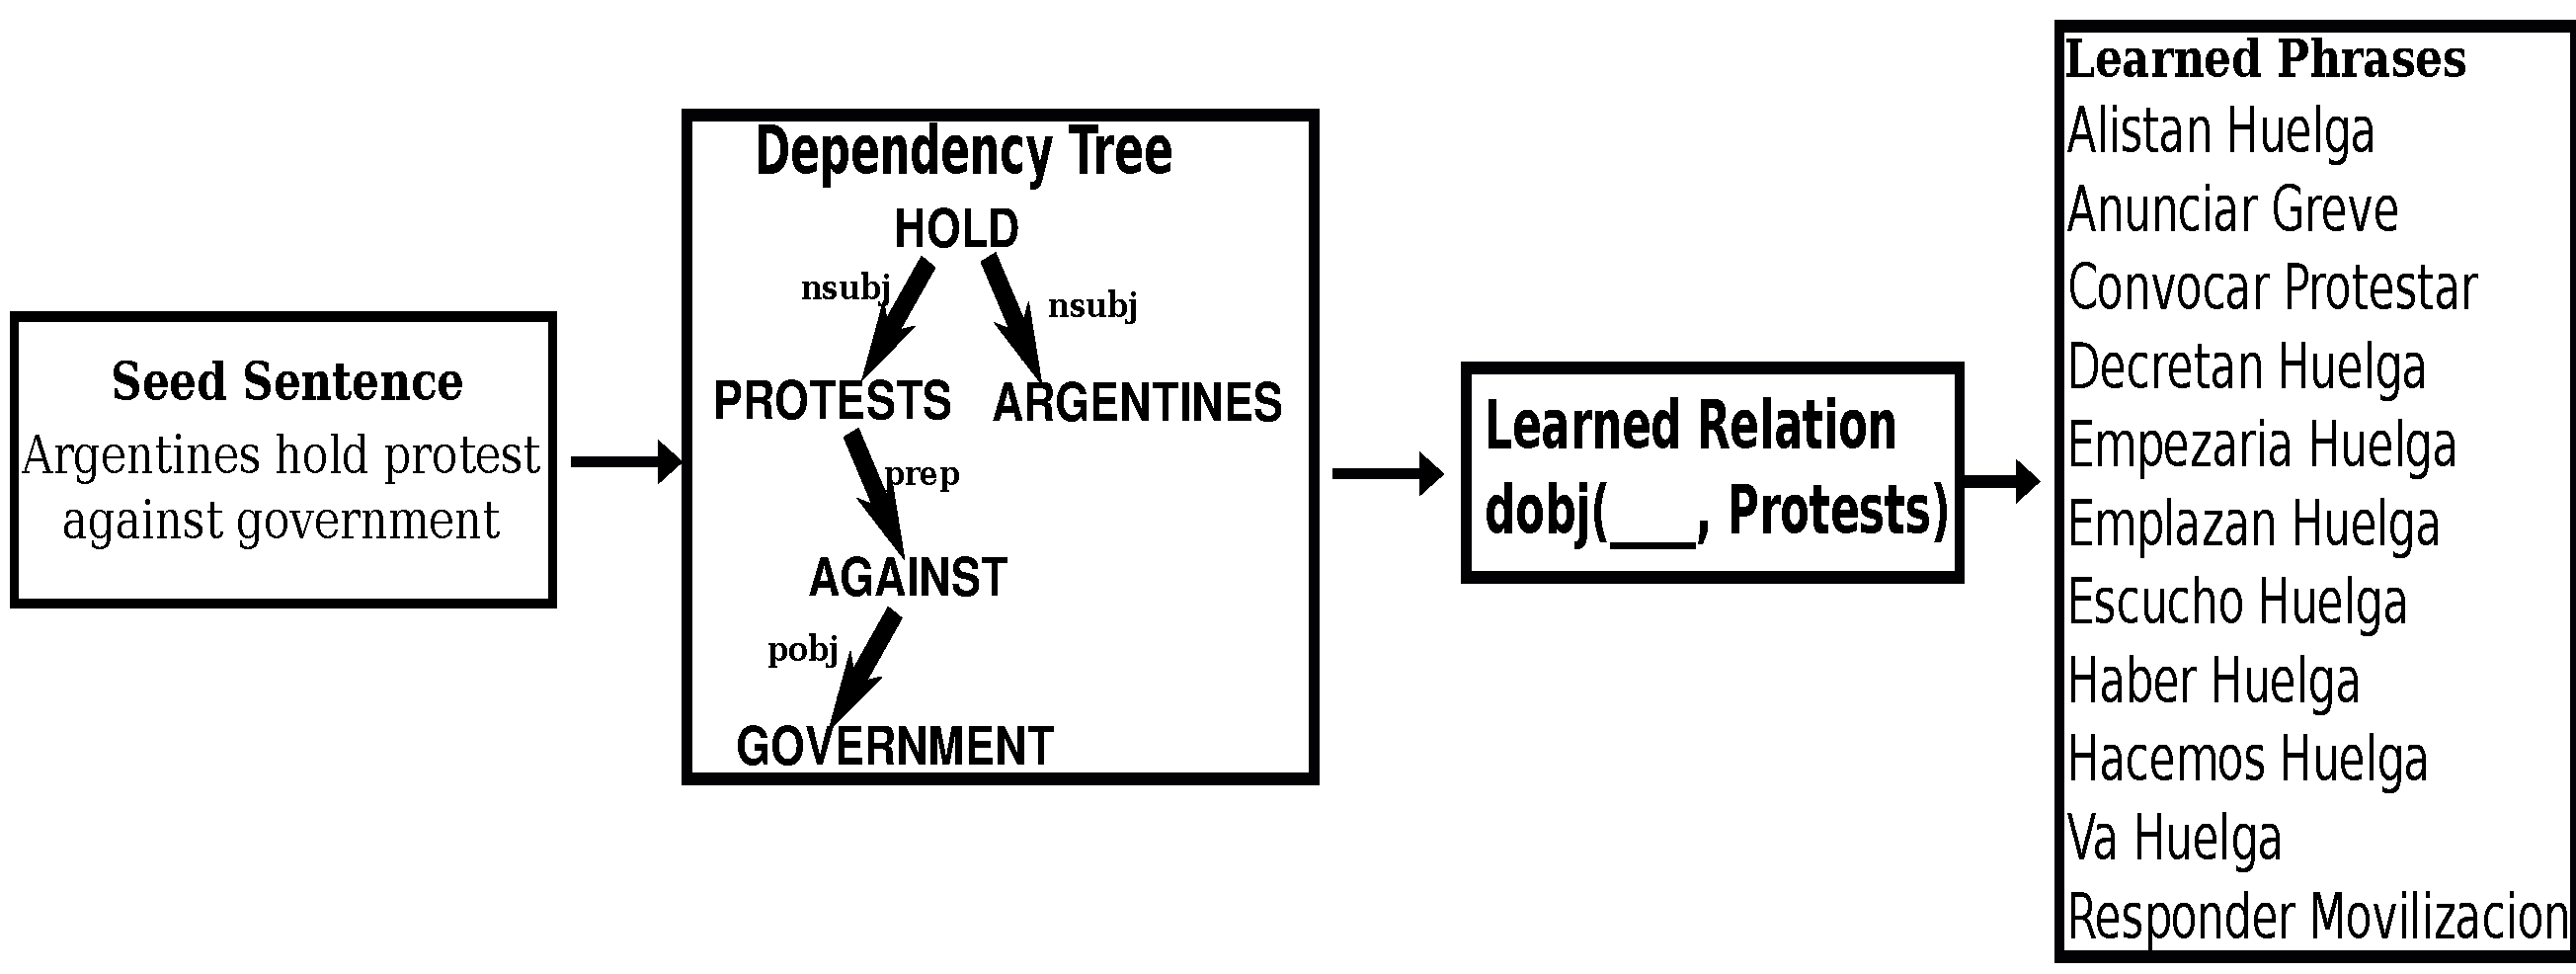
\includegraphics[scale=0.4]{figures/phraseLearning}
\caption{An example of phrase learning for detecting planned protests.}
\label{fig:phraselearning}
\end{figure}

\section{Geocoding}
\label{subsection:geocoding}
After linguistic preprocessing and suitable phrase filtering,
messages are geocoded with a
specification of the geographical focus of the text---specified as a
city, state, country triple---that indicates the locality that the
text is about. We make use of different geocoding methodologies
for Twitter messages, for Facebook Events pages, and for news articles and blogs.
These are described below.

\subsection{Twitter}
For tweets, the geo-focus of the message is generated by a fairly
simple set of heuristics.  In particular, Twitter
geocoding is achieved by first considering the most reliable but least
available source, the geotag (latitude, longitude) of the tweet itself (this is available
for about 10\% of our sample from Twitter). This provide an exact
geographic location that can be reverse geocoded into a place name
and used as the geo-focus. We find the nearest geo-coded point in
our extended gazetteer (using a kd-tree data structure) for this
purpose. If the tweet is not geocoded, we consider Twitter {\it places}
metadata and use place names present in these metadata fields to
geocode the place names into geographical coordinates. Finally, if
none of this is available, we consider the text fields contained in
the user profile (location, description) as well as the tweet text
itself to find mentions of relevant locations.  Additional toponym disambiguiation heuristics are used to
identify the actual referent of the mention.

\subsection{Facebook}
Similar methods are used to geocode event data extracted from Facebook event pages.  
Since only Facebook events that have a venue are used and since the
 venue of a Facebook event generally specifies a latitude, longitude, and physical address information, 
identifying the location is a fairly trivial task.  In cases where only latitude and longitude are given, 
we apply reverse-geocoding mechanisms similar to those used for Twitter.

\subsection{News and Blogs}
For longer articles such as news articles, the geo-focus of the message is identified using much more complex methods
To extract the protest location from news articles, we use PSL to build probabilistic models that infer the intended
location of a protest by 
weighing evidence coming from the Basis entity extractions and information in the World Gazeteer. 

The primary rules in the model encode the effect that Basis-extracted location strings that match to gazatteer 
aliases are indicators of the article's location, whether they be country, state, or city aliases. 
Each of these implications is conjuncted with an prior for ambiguous, overloaded aliases that is 
proportional to the population of the gazetteer location. For example, if the string ``Los Angeles'' appears in the article, 
it could refer to either Los Angeles, California, or Los \'{A}ngeles in Argentina or Chile. Given no other information,
our model would infer a higher truth value for the article referring to Los Angeles, California, because it 
has a much higher population than the other options. 
\begin{flalign*}
    ENTITY&(L, location) \softand REFERSTO(L, locID) &\\
                        &\rightarrow PSLLOCATION(Article, locID) &
\end{flalign*}

\begin{flalign*}
    ENTITY&(C, location) \softand IsCountry(C) &\\
                        &\rightarrow ArticleCountry(Article, C) &
\end{flalign*}

\begin{flalign*}
    ENTITY&(S, location) \softand IsState(S)&\\
                            &\rightarrow ArticleState(Article, S)&
\end{flalign*}

\noindent
(Note that the above are not deterministic rules; e.g., they do not use the logical conjunction $\wedge$ but rather the
Lukasiewicz t-norm based relaxation $\softand$. Further, these rules do not fire deterministically but are instead
simultaneously solved for satisfying assignments as described in Section~\ref{section:PSL}.)

The secondary rules, which are given half the weight of the primary rules, perform the same mapping of extracted strings 
to gazetteer aliases, but for extracted persons and organizations. Strings describing persons and 
organizations often include location clues (e.g., ``mayor of Buenos Aires''), but intuition suggests 
the correlation between the article's location and these clues may be lower than with location strings. 
\begin{flalign*}
    ENTITY&(O, organization) \softand REFERSTO(O, locID)&\\
                            &\rightarrow PSLLOCATION(Article, locID) &
\end{flalign*}

\begin{flalign*}
    ENTITY&(O, organization) \softand IsCountry(O)&\\
        &\rightarrow ArticleCountry(Article, O)&
\end{flalign*}

\begin{flalign*}
    ENTITY&(O, organization) \softand IsState(O)&\\
          &\rightarrow ArticleState(Article, O) &
\end{flalign*}
Finally, the model includes rules and constraints to require consistency between the different levels of geolocation, 
making the model place higher probability on states with its city contained in its state, which is 
contained in its country. As a post-processing step, we enforce this consistency explicitly by using the 
inferred city and its enclosing state and country, but adding these rules into the model makes the 
probabilistic inference prefer consistent predictions, enabling it to combine evidence at all levels.
As an example of how PSL aids in location identification, the example from Fig.~\ref{pp_example}
is revisited in Fig.~\ref{fig:psl_example}. 
\begin{flalign*}
    PSLLOCATION&(Article, locID) \softand Country(locID, C)&\\
               &\rightarrow ArticleCountry(Article, C)&
\end{flalign*}

\begin{flalign*}
    PSLLOCATION&(Article, locID) \softand Admin1(locID, S)&\\
               &\rightarrow ArticleState(Article, S)&
\end{flalign*}

\begin{figure*}
    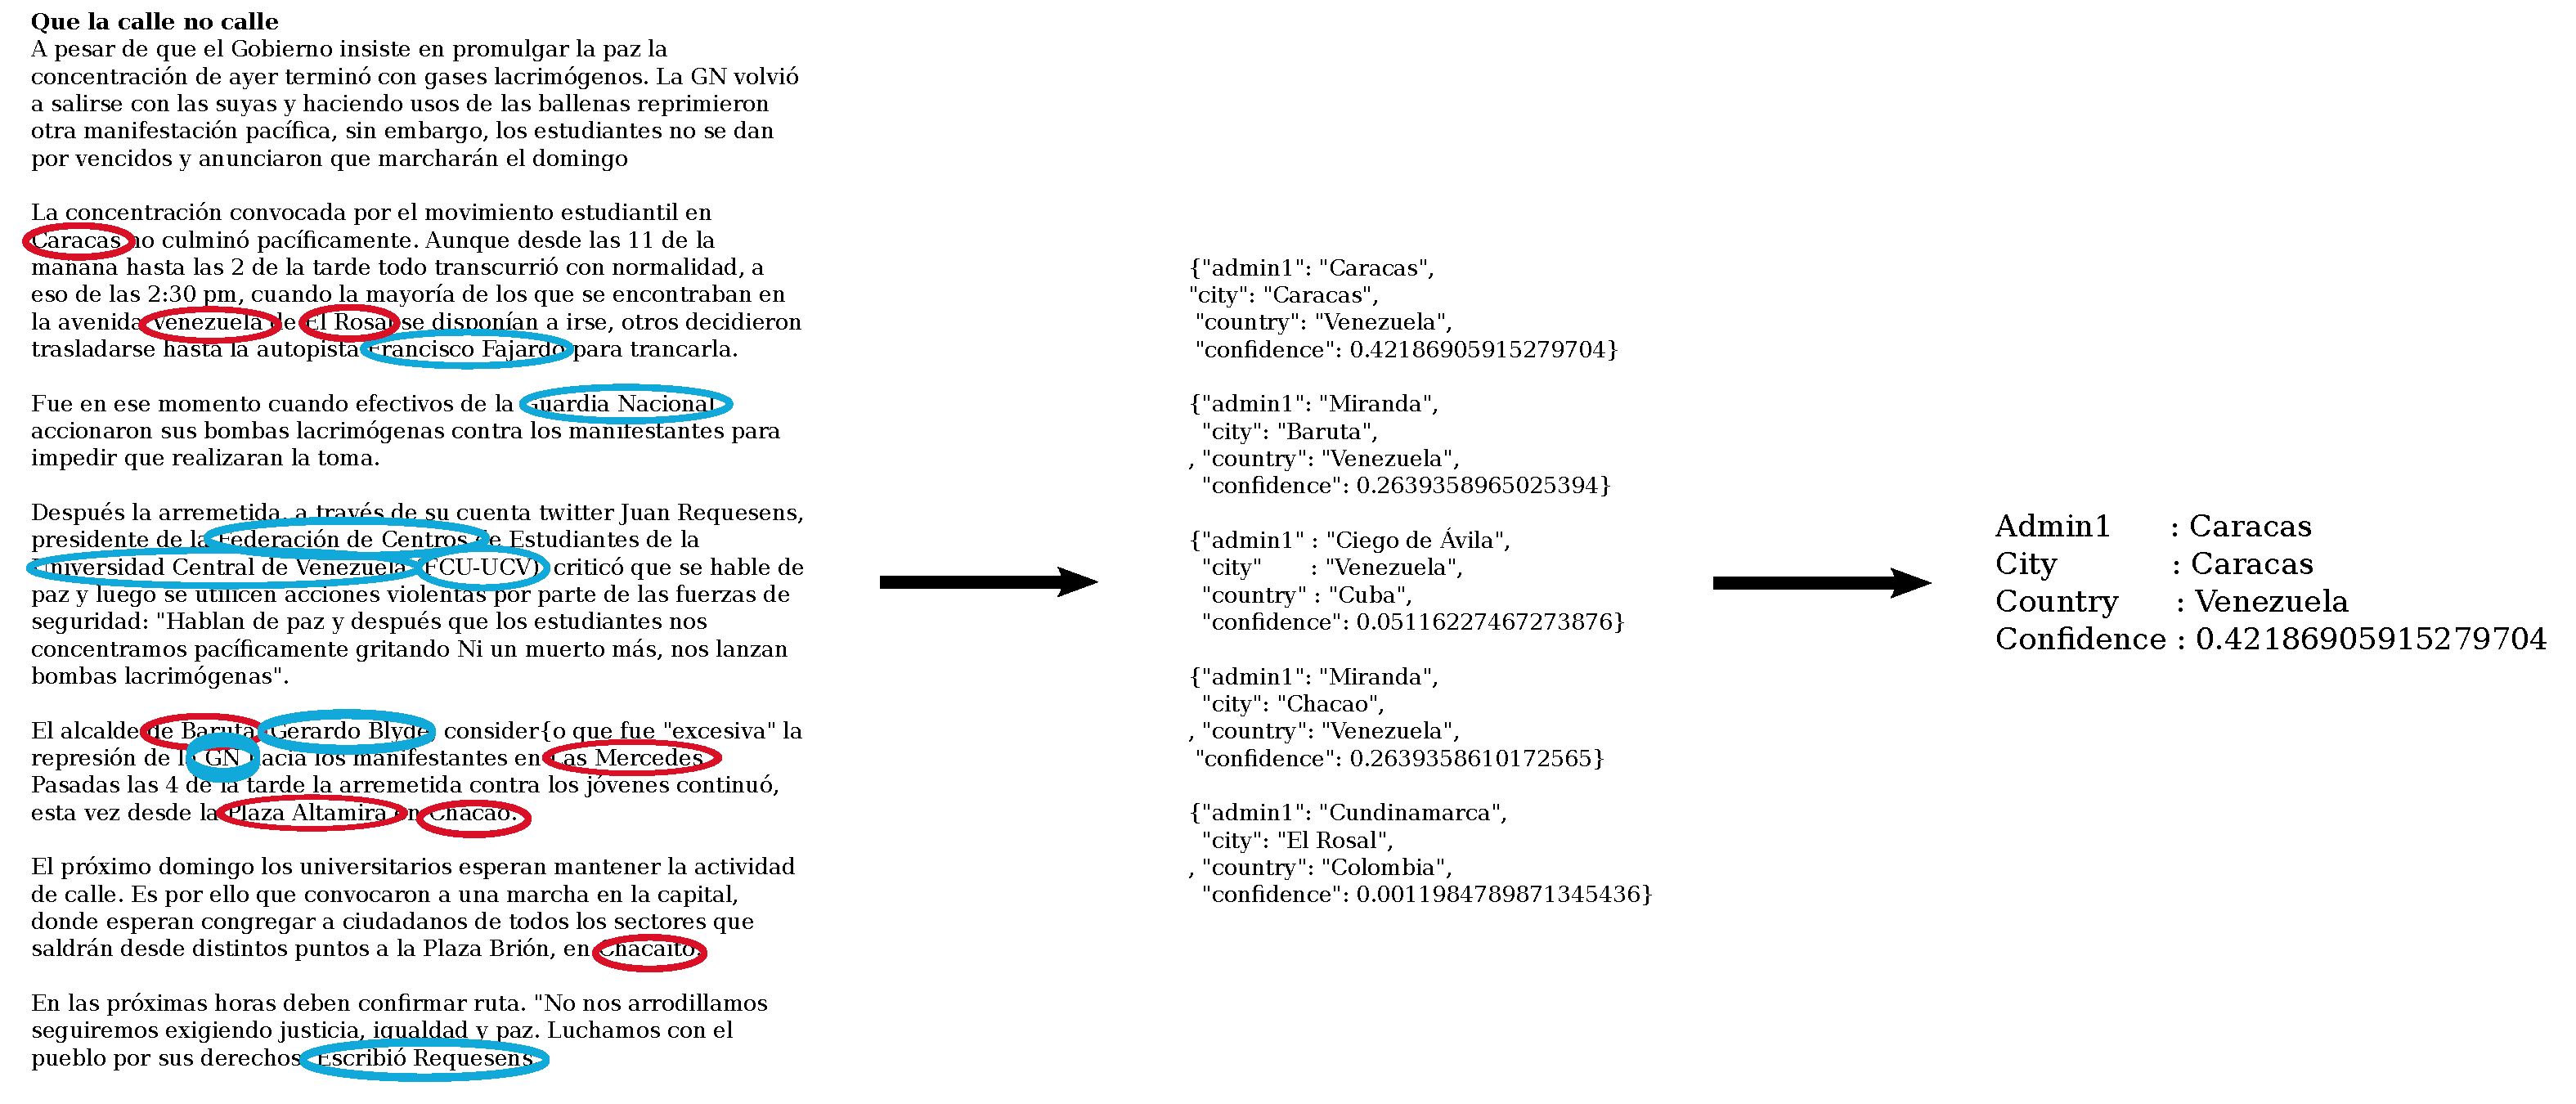
\includegraphics[width=\textwidth]{psl_pipeline2}
    \caption{An example of location inference using PSL. Red circles denote named entities identified as locations and blue denotes other types of entities. The 
article describes students planning a march on Sunday.
It identifies multiple locations, e.g., Chacao, El Roso, and the Francisco Fajardo highway where protests have been happening.
There is also a reference to a quote by the mayor of Baruto.
Mentions of such multiple locations are resolved using our PSL program to the intended location, here Caracas.}
    \label{fig:psl_example}
\end{figure*}

%%!TEX root = ../plannedprotest.tex

%\iffalse
%To extract the protest location from news articles, we use \emph{probabilistic soft logic} (PSL) \cite{broecheler:uai10} to build a model that performs robust, probabilistic inference given noisy signals. PSL takes a set of weighted, logic-like rules and converts them into a continuous probability distribution over the unknown truth values of logical facts. These truth values in PSL are relaxed into the $[0,1]$ interval. We use this mechanism to build a model that infers the semantic location of an article by weighing evidence coming from the Basis entity extractions and information in the World Gazatteer. 
%
%The primary rules in the model encode the effect that Basis-extracted location strings that match to gazatteer aliases are indicators of the article's location, whether they be country, state, or city aliases. Each of these implications is conjuncted with an prior for ambiguous, overloaded aliases that is proportional to the population of the gazetteer location. For example, if the string ``Los Angeles'' appears in the article, it could refer to either Los Angeles, California, or Los \'{A}ngeles in Argentina or Chile. Given no other information, our model would infer a higher truth value for the article referring to Los Angeles, California, because it has a much higher population than the other options. 
%
%The secondary rules, which are given half the weight of the primary rules, perform the same mapping of extracted strings to gazetteer aliases, but for extracted persons and organizations. Strings describing persons and organizations often include location clues (e.g., ``mayor of Buenos Aires''), but intuition suggests the correlation between the article's location and these clues may be lower than with location strings. 
%
%Finally, the model includes rules and constraints to require consistency between the different levels of geolocation, making the model place higher probability on states with its city contained in its state, which is contained in its country. As a post-processing step, we enforce this consistency explicitly by using the inferred city and its enclosing state and country, but adding these rules into the model makes the probabilistic inference prefer consistent predictions, enabling it to combine evidence at all levels.
%\fi

In this section, we briefly describe probabilistic soft logic (PSL)~\cite{kimmig2012short}, a key
component of our geocoding strategy described later.
PSL is a framework for collective probabilistic reasoning on relational domains.
PSL models have been developed in various domains, including collective classification~\cite{broecheler2010computing}, 
ontology alignment~\cite{brocheler2012probabilistic}, personalized medicine~\cite{bach2010decision}, 
opinion diffusion~\cite{bach2012scaling} , trust in social networks~\cite{huang2012probabilistic}, and graph 
summarization~\cite{memory2012graph}.
PSL represents the domain of interest as logical atoms.
It uses first order logic rules to capture the dependency structure of the domain, based on which it builds a joint probabilistic model over all atoms.
Instead of hard truth values of $0$ (false) and $1$ (true), PSL uses soft truth values relaxing the truth vlaues to the interval $[0,1]$.
The logical connectives are adapted accordingly.
This makes it easy to incorporate similarity or distance functions.

User defined \emph{predicates} are used to encode the relationships and attributes and \emph{rules} capture the  dependencies and constraints.
Each rule's antecedent is a conjunction of atoms and its consequent is a dis-junction. 
The rules can also labeled with non negative weights which are used during the inference process.
The set of predicates and weighted rules thus make up a PSL program where known truth values of ground atoms derived from observed data and unknown truth values for the remaining atoms are learned using the PSL inference.

Given a set of atoms 
$\ell = \{\ell_1,\ldots,\ell_n\}$,
an interpretation defined as 
$I : \ell \rightarrow [0,1]^n$
is a mapping from atoms to soft truth values.
PSL defines a probability distribution over all such interpretaions such that those that satisfy more ground rules are more probable.
\emph{Lukasiewicz t-norm} and its corresponding co-norm are used for defining relaxations of the logical AND and OR respectively to determine the degree to which a ground rule is satisfied.
Given an interpretation $\mathit{I}$, PSL defines the formulas for the relaxation of the logical conjunction ($\wedge$), disjunction ($\vee$), and negation ($\neg$) as follows:

\begin{align*}
\ell_1 \softand \ell_2 &= \max\{0, I(\ell_1) + I(\ell_2) - 1\},\\
\ell_1 \softor \ell_2 &= \min\{I(\ell_1) + I(\ell_2), 1\},\\
\softneg l_1 &= 1 - I(\ell_1),
\end{align*}  

The interpretation $\mathit{I}$ determines whether the rules is satisfied, if not, the \emph{distance to satisfaction}.
A rule $\mathit{r} \equiv \mathit{r_{body}} \rightarrow \mathit{r_{head}} $  is satisfied if and only if the truth value of head is at least that of the body. The rule's distance to satisfaction measures the degree to which this condition is violated.
 \newline
\begin{center} 
 $\mathit{d_r}(\mathit{I}) =$ max\{0,$\mathit{I(r_{body})} - \mathit{I(r_{head})}$\}
 \end{center}

PSL then induces a probability distribution over possible interpretations $\mathit{I}$ over the given set of ground atoms $\mathit{l} $ in the domain. 
If $\mathit{R}$ is the set of all ground rules that are instances of a rule from the system and uses only the atoms in  $\mathit{I}$ then,
the probability density function $\mathit{f}$ over $\mathit{I}$ is defined as
\begin{equation}
\label{eq:contimn1}
    f (I) = \frac{1}{Z} \text{exp}[-\sum_{r\in R} \lambda_r (d_r(I))^p]
\end{equation}
\begin{equation}
\label{eq:contimn2}
	Z = \int_{I} \text{exp} [ -\sum_{r\in R} \lambda_r (d_r(I))^p ]
\end{equation}
where~$\lambda_r$ is the weight of the rule~$r$, $Z$ is the continuous version of the normalization constant used in discrete Markov random fields, and ~$p \in \{1, 2\}$ provides a choice between two different loss functions, linear and quadratic.
The values of the atoms can be further restricted by providing linear equality and inequality constraints allowing one to encode functional constraints from the domain. 

PSL provides for two kinds of inferences:
(a) most probable explanation and (b) calculation of the marginal distributions. 
In the MPE inference given a partial interpretation with grounded atoms based on observed evidence, the PSL program infers the truth values for the unobserved atoms satisfying the most likely interpretation. 
In the second setting, given ground truth data for all atoms we can learn the weights for the rules in our PSL program.

\iffalse Most news articles and blog posts mention multiple locations, e.g.,
the location of reporting, the location of the incident, and locations corresponding
to the hometown of the newspaper. We developed a probabilistic reasoning
engine using probabilistic soft logic (PSL)
to infer the most likely city, state and country which is the main geographic focus the article.The PSL geocoder combines various types of evidence, such as named entities
such as locations, persons, and organizations identified by RLP, as
well as common names and aliases and populations of known
locations. These diverse types of evidence are used in weighted rules
that prioritize their influence on the PSL model's location
prediction. For example, extracted location tokens are strong
indicators of the content location of an article, while organization
and person names containing location names are weaker but still
informative signals; the rules corresponding to these evidence types
are weighted accordingly.

The methodology is similar to {\em Web-a-where: Geo-Tagging Web Content}.
\fi 

%\begin{figure}
%    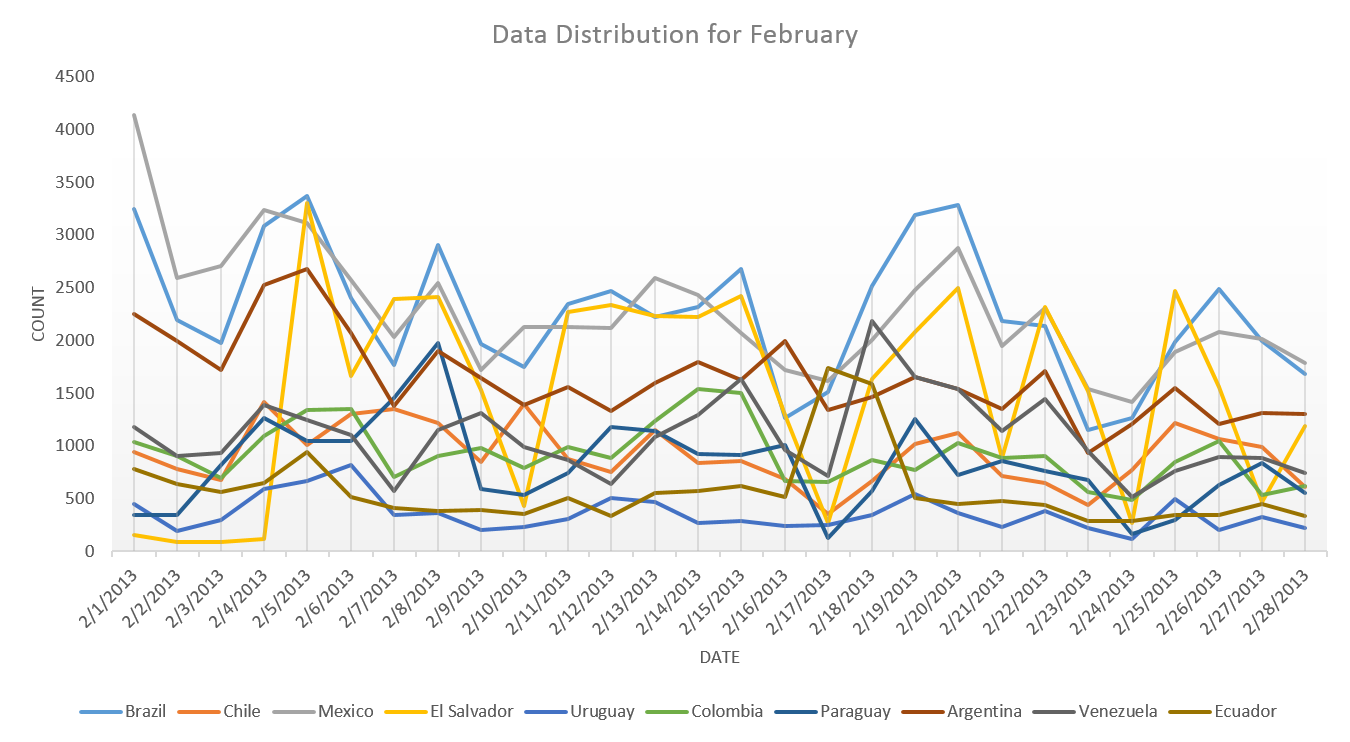
\includegraphics[width=0.5\textwidth]{rssdistribution}
%    \caption{Rate of Arrival of News/Blogs}
%    \label{fig:rssdistribution}
%\end{figure}
%
\subsection{Warning Generation}
After being subject to the preprocessing steps, above, all documents
that are identified as containing a key phrase are further filtered by
searching for the presence a future date in the passage containing the
key phrase and for the existence of an identified geographical focus for the text.
Documents that meet all these critera are used as the basis for a warning about a
planned civil unrest event (Twitter postings are only used as the basis for a warning
if the tweet is re-tweeted at least five times). 
A warning is generated for the date indicated by the future date
expression and the location which is the geographical focus of the
document.  
In the case of Facebook, an event page is considered to be good evidence for an alert if
there are more attendees for the event than rejects.  The date and
location are read off from the event page directly.


\chapter{Experiments}
\markright{Sathappan Muthiah \hfill Chapter 6. Experiments \hfill}
We evaluate our planned protest detection system
using metrics similar to those described by Ramakrishnan et al.~\cite{emberskdd} in evaluating their work.
Given a set of alerts issued by the system and the GSR comprising actual protest incidents, we aim to identify
a correspondence between the two sets via a bipartite matching.
An alert can be matched to a GSR event only if i) they are both issued for the same country, 
ii) the alert's predicted location and the event's reported location are within 300km of each
other (the distance offset), and iii) the forecasted event date is within a given interval of the true event date (the date offset).
Once these inclusion criteria apply, the quality score (QS) of the match is defined as a combination of the
location score (LS) and date score (DS):
\begin{equation}
    \operatorname{QS}= (LS + DS)*2
\end{equation}
\noindent
where
\begin{equation}
    \operatorname{LS}=1 - \frac{\min(\textrm{distance offset}, 300)}{300}
\end{equation}
and 
\begin{equation}
    \operatorname{DS}=1 - \frac{\min(\textrm{date offset}, \operatorname{INTERVAL})}{\operatorname{INTERVAL}}
\end{equation}
Here, we explore $\operatorname{INTERVAL}$ values from $0$ to $7$.
if an alert (conversely, GSR event) cannot be matched to any GSR event (alert, respectively), these unmatched
alerts (and events) will negatively impact the precision (and recall) of the system. The lead time,
for a matched alert-event pair,
is calculated as the difference between the date on which the forecast was made and the date on which the event
was reported (this should not be confused with the date score, which is the difference between the
predicted event date and the actual event date). Lead time concerns itself with reporting and forecasting, whereas
the date score is concerned with quality or accuracy.

We conduct a series of experiments to evaluate the performance of our system.\\

\begin{figure*}
\centering
\begin{subfigure}{\columnwidth}
  \centering
  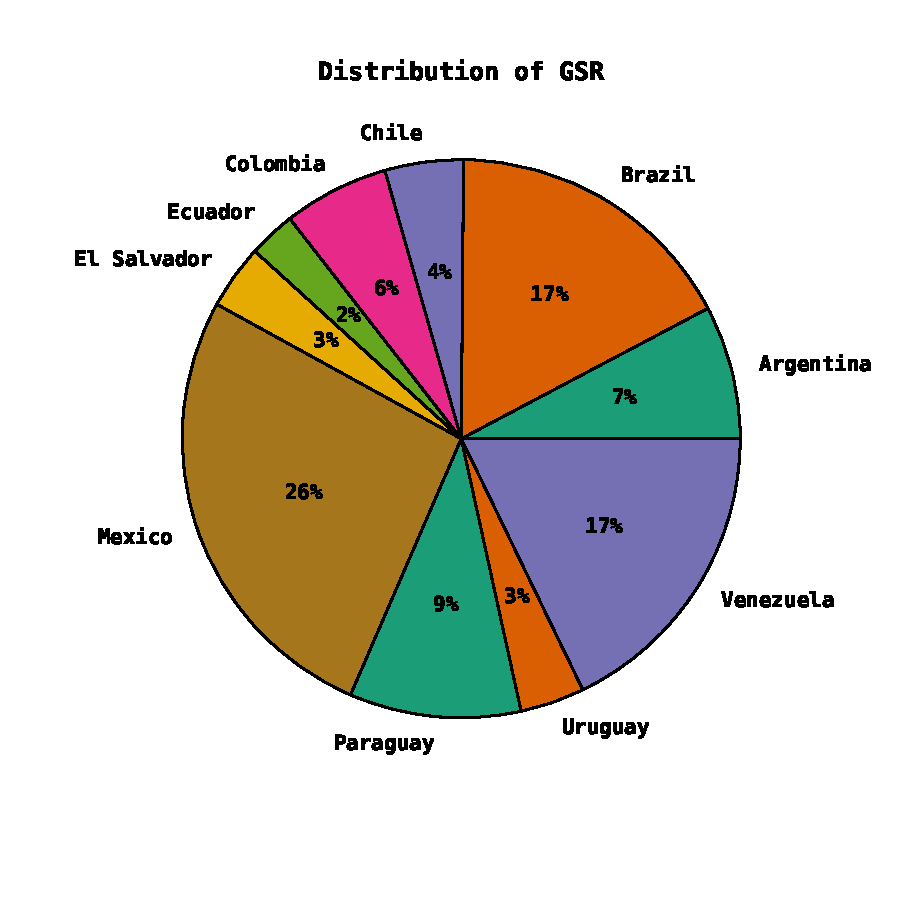
\includegraphics[scale=0.7]{gsr_distribution}
  \caption{GSR distribution from 2012-11 to 2014-03.}
  \label{fig:gsrdistribution}
\end{subfigure}
\begin{subfigure}{\columnwidth}
  \centering
  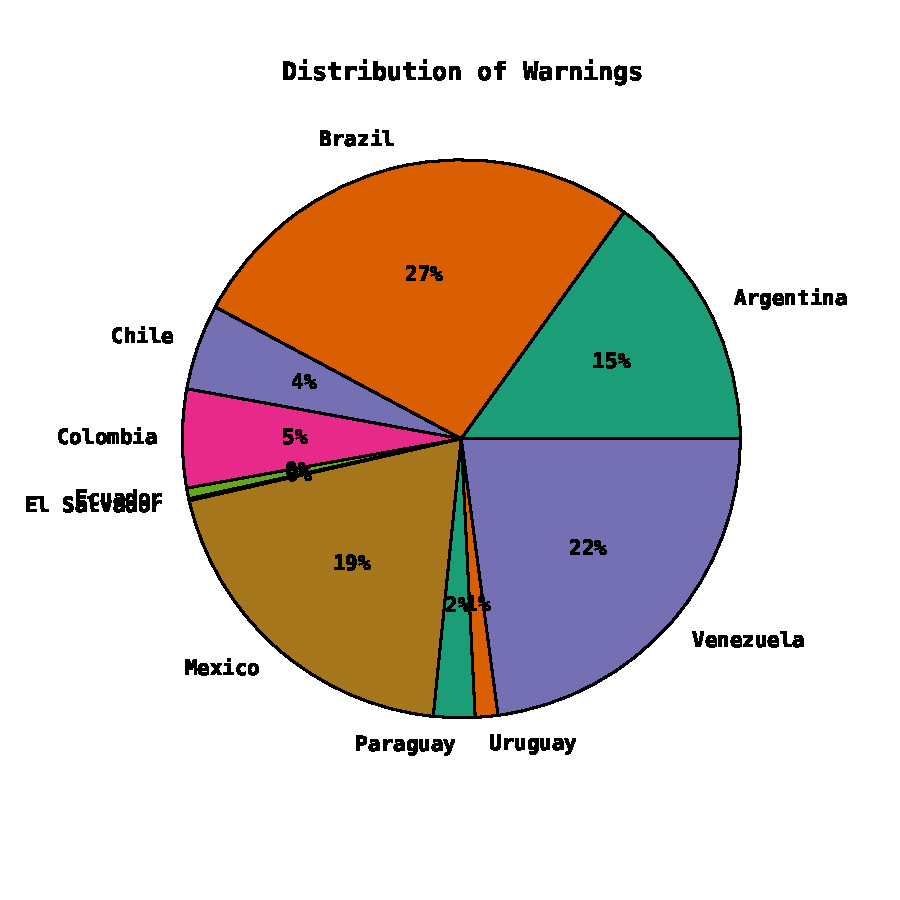
\includegraphics[scale=.7]{pp_dist}
  \caption{Alerts distribution from 2012-11 to 2014-03.}
  \label{fig:ppdistribution}
\end{subfigure}
\caption{Distribution of alerts and GSR events across the countries studied in this paper.}
\label{fig:distribution}
\end{figure*}

\noindent
{\bf Distribution of protests detected by the system compared with the
actual distribution of protests in the GSR?}
Fig.~\ref{fig:distribution} reveals pie charts of both distributions. As shown, Mexico, Brazil, and Venezuela
experience the lion's share of protests in our region of interest, and the protests detected also match these modes
although not the specific percentages. The smaller countries like Ecuador, El Salvador, and Uruguay do experience
protests but which are not as prominently detected as those for other countries; we attribute this to their smaller
social media footprint (relative to countries like Brazil and Venezuela).\\
\begin{table*}[tb!]
    \tiny
    \centering
    \caption[Country-wise breakdown of forecasting performance for different data sources.]{
QS=Quality Score; Pr=Precision; Rec=Recall; LT=Lead Time.
AR=Argentina; BR=Brazil; CL=Chile; CO=Colombia; EC=Ecuador;SV=El Salvador; MX=Mexico; PY=Paraguay; UY=Uruguay; VE=Venezuela. A $-$ indicates that the source did not produce any warnings for that country in the studied period.}
    \label{tb:sourcewisecomparison}
    \begin{tabular}{|*{17}{c|}}
        \hline
        & \multicolumn{4}{ |c| }{News/Blogs} & \multicolumn{4}{ |c| }{Twitter} & \multicolumn{4}{ |c| }{Facebook} & \multicolumn{4}{ |c| }{Combined}\\
        \hline
         & QS & Pr. & Rec. &LT & QS & Pr. & Rec. & LT & QS & Pr. & Rec. & LT & QS & Pr. & Rec. & LT\\
        \hline
        AR &3.14&0.32&0.69&3.94&3.52&{\bf0.78}&0.14&3.14&{\bf3.70}&0.50&0.04&3.00&3.02&0.36&{\bf0.80}&{\bf4.50}\\
        BR &3.14&0.48&0.54&{\bf5.85}&-&-&-&-&{\bf3.62}&{\bf0.76}&0.18&2.46&3.28&0.49&{\bf0.65}&5.15\\
        CL &3.06&0.91&0.67&5.40&{\bf3.52}&{\bf1.00}&0.23&4.29&-&-&-&-&3.16&0.83&{\bf0.80}&{\bf5.92}\\
        CO &2.74&0.90&0.56&{\bf7.44}&3.30&{\bf1.00}&0.15&2.43&{\bf4.00}&{\bf1.00}&0.02&2.00&2.88&0.84&{\bf0.65}&6.47\\
        EC &-&-&-&-&{\bf2.32}&{\bf1.00}&{\bf0.06}&{\bf17.00}&-&-&-&-&{\bf2.32}&{\bf0.50}&{\bf0.06}&{\bf17.00}\\
        MX &2.96&0.88&0.25&{\bf3.69}&3.14&{\bf1.00}&0.02&1.43&{\bf3.72}&0.67&0.01&2.00&3.00&0.87&{\bf0.27}&3.51\\
        SV &{\bf3.22}&{\bf1.00}&{\bf0.03}&{\bf1.0}&-&-&-&-&-&-&-&-&{\bf3.22}&{\bf1.0}&{\bf0.03}&{\bf1.0}\\
        PY &3.38&{\bf1.00}&{\bf0.16}&9.11&3.84&{\bf1.00}&0.04&{\bf11.40}&3.96&{\bf1.00}&0.01&2.00&3.60&0.96&{\bf0.20}&9.35\\
        UY &{\bf3.24}&{\bf1.00}&{\bf0.29}&{\bf2.40}&-&-&-&-&-&-&-&-&3.24&{\bf1.00}&{\bf0.29}&3.24\\
        VE &{\bf3.80}&{\bf1.00}&0.36&{\bf3.27}&3.68&0.97&0.33&2.39&-&-&-&-&3.64&0.99&{\bf0.69}&2.88\\
        ALL &3.34&0.69&0.35&{\bf4.57}&3.62&{\bf0.97}&0.15&2.82&3.66&0.74&0.03&2.44&3.36&0.73&{\bf0.51}&4.08\\
        \hline
    \end{tabular}
\end{table*}

\begin{figure*}
  \centering
  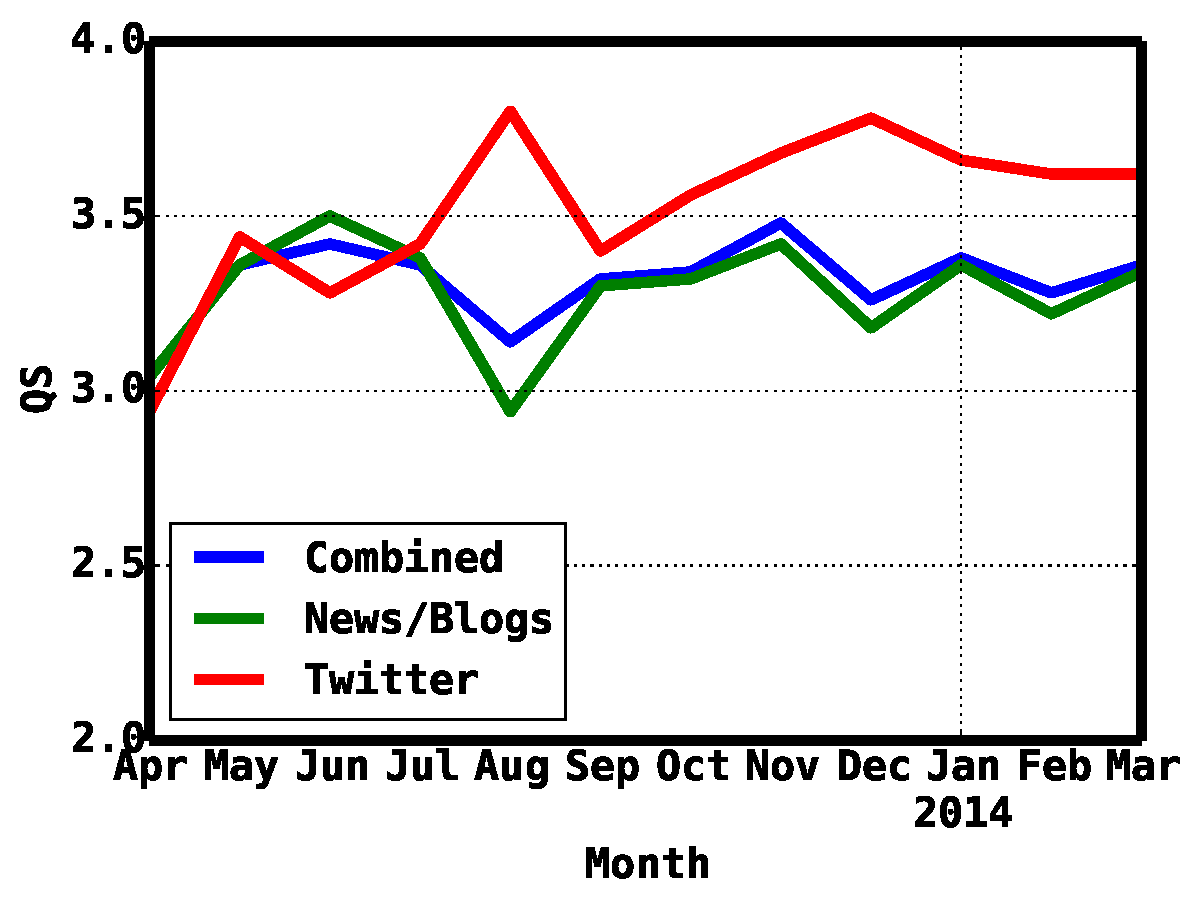
\includegraphics[scale=0.6]{monthlyqs}
  \caption{Quality Score over the months}
  \label{fig:monthlyqs}
\end{figure*}

\noindent
{\bf Are there country-specific selective superiorities for the different data sources considered here?}
Table~\ref{tb:sourcewisecomparison} presents a breakdown of perfomance, country-wise and source-wise, of
our approach for a recent month, viz. March 2014.
It is clear that the multiple data sources are necessary to achieve a high recall and that by and large
these sources are providing mutually exclusive alerts. (Note also that some data sources do not produce alerts for specific
countries.) Between Twitter and Facebook, the former is a better
source of alerts for countries like Chile and the latter is a better source for Argentina, Brazil, Colombia, and Mexico.
News and blogs achieve higher recall than social media sources indicating that most plans for protests are announced
in established media. They are also
higher quality sources for alerts in countries like El Salvador, Paraguay, and Uruguay.
Finally, note that news and blogs offer a much higher lead time (4.57 days)
as compared to that for Facebook (2.44 days) or for Twitter (2.82 days). The quality scores are
further broken down in Table~\ref{tb:modelwisecomparison} into their date and location components.
A longitudunal perspective on quality scores is
given in Fig.~\ref{fig:monthlyqs}. Note that in general Twitter tends to have a higher quality score
as multiple re-tweets of future event mentions is a direct indicator of the popularity of an event as
well as the intent of people to join an event.
In contrast, mentions of future events in news do not directly shed any insight into popularity or people's
support for the event's causes.\\

\begin{table*} %[tb!]
\centering
\caption[Comparing the location and date scores of different sources in specific countries.]{
AR=Argentina; BR=Brazil; CL=Chile; CO=Colombia; EC=Ecuador;SV=El Salvador; MX=Mexico; PY=Paraguay; UY=Uruguay; VE=Venezuela. A $-$ indicates that the source did not produce any warnings for that country in the studied period.}
\label{tb:modelwisecomparison}
\begin{tabular}{||l|*{17}{c|}}
\hline
Source& & AR & BR & CL & CO & EC & SV & MX & PY & UY & VE & All\\
\hline
\multirow{2}{*}{News/Blogs} &LS &0.82&0.76&0.75&0.60&-&{\bf0.75}&0.66&0.79&{\bf0.79}&{\bf0.95}&0.81\\
                            &DS&0.75&0.81&0.78&0.77&-&{\bf0.86}&0.82&0.90&{\bf0.83}&{\bf0.95}&0.86\\
\hline
\multirow{2}{*}{Facebook} &LS &{\bf1.0}&{\bf0.92}&-&{\bf1.00}&-&-&{\bf0.86}&{\bf0.98}&-&-&{\bf0.93}\\
                          &DS&0.85&{\bf0.89}&-&{\bf1.00}&-&-&{\bf1.00}&{\bf1.00}&-&-&0.90\\
\hline
\multirow{2}{*}{Twitter} &LS &0.88&-&{\bf0.84}&0.81&{\bf0.45}&-&0.71&{\bf0.98}&-&0.91&0.89\\
                         &DS&{\bf0.88}&-&{\bf0.92}&0.84&{\bf0.71}&-&0.86&0.94&-&0.93&{\bf0.92}\\
\hline
\end{tabular}
\end{table*}


\begin{figure*}
  \centering
  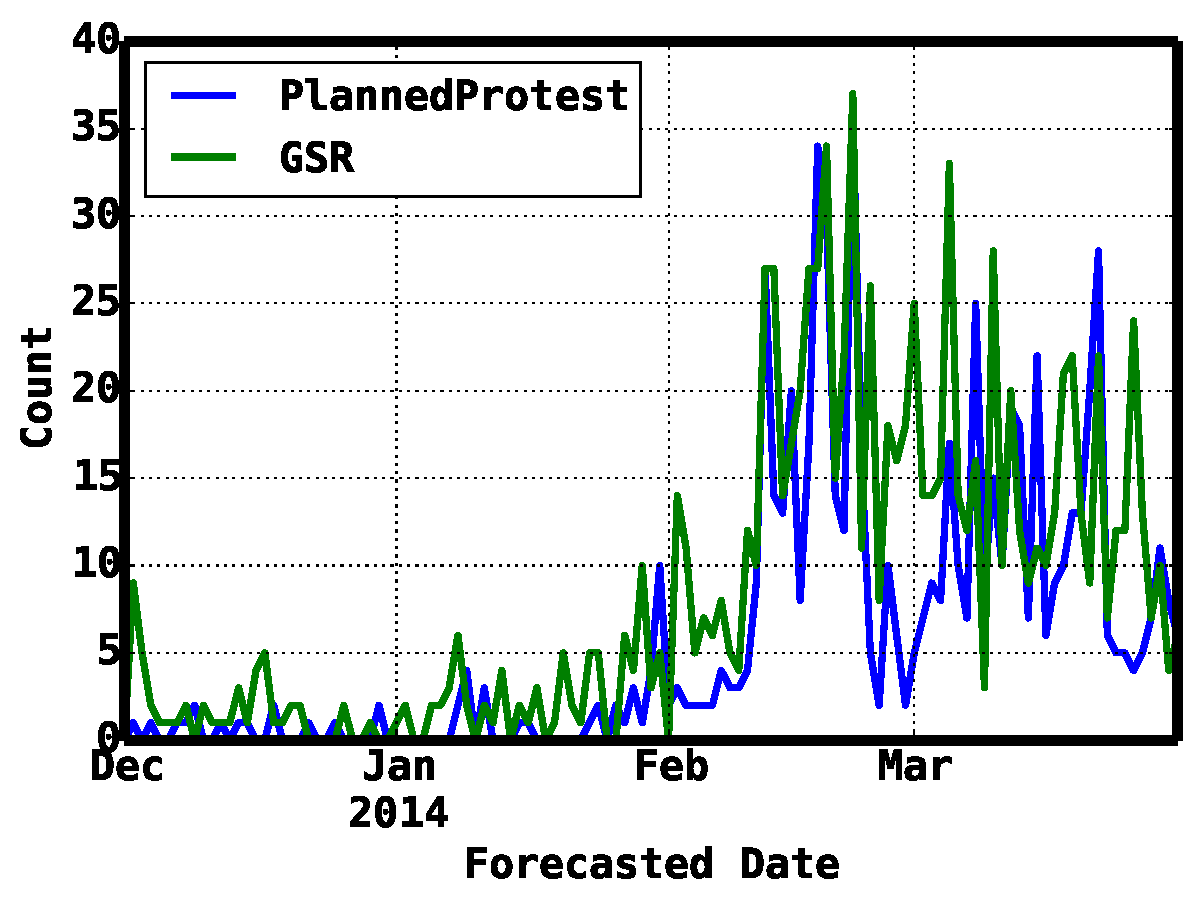
\includegraphics[scale=0.6]{venezuela}
  \caption{Venezuelan Protests}
  \label{fig:venezuela_feb}
\end{figure*}
\begin{figure*}
  \centering
  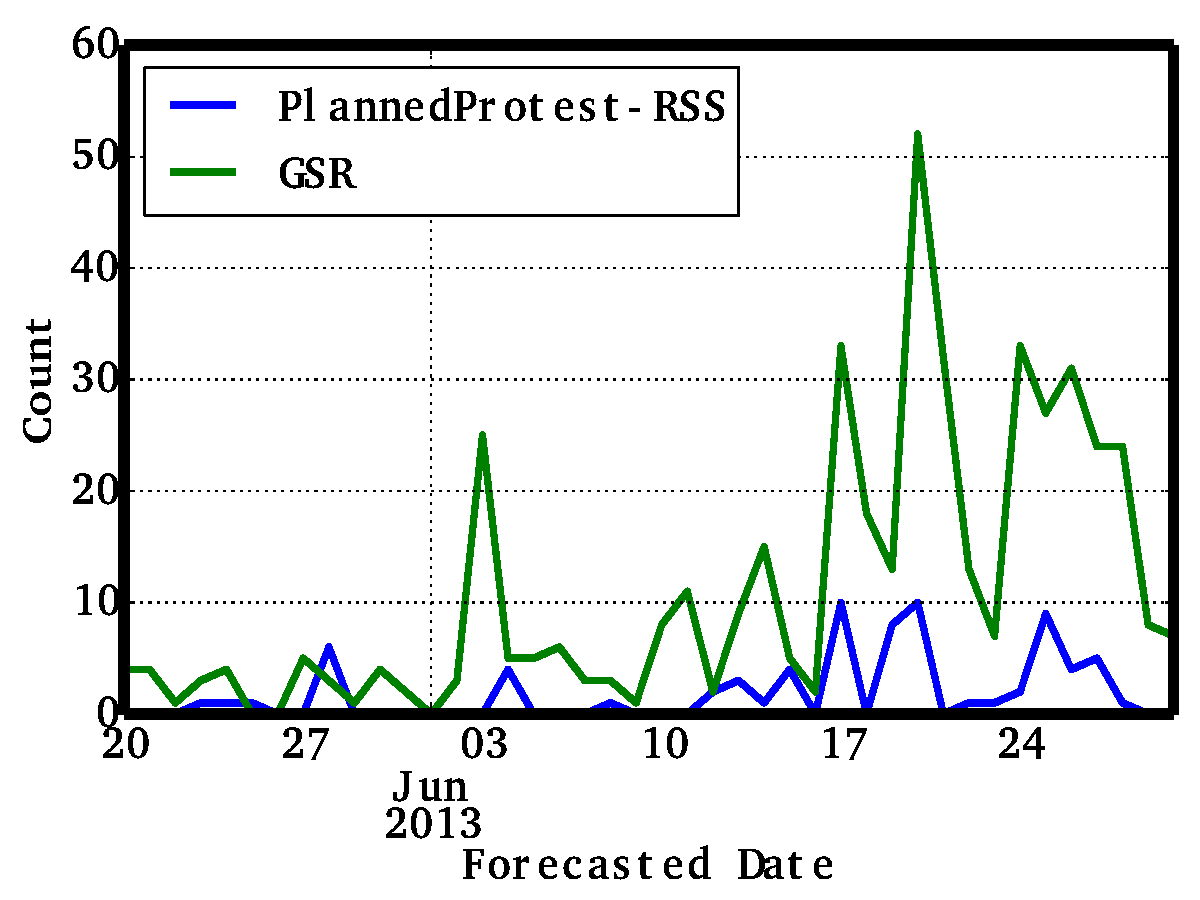
\includegraphics[scale=0.6]{brazil_june}
  \caption{System Performance during Brazilian Spring}
  \label{fig:brazil_june}
\end{figure*}
\noindent
{\bf How did our system fare in detecting key country-wide protests?}
The recent Venezuelan protests against President Nicolas Maduro and the Brazilian Protests during June 2013 against bus fare hike were two significant protests during our period of evaluation. Fig.~\ref{fig:venezuela_feb} and
Fig.~\ref{fig:brazil_june} describe our performance under these two situations illustrating the count
of protests detected against the GSR. Notice that our system was able to 
identify the Venezuelan protests much better than the Brazilian protests. This is because there was a significant amount
of spontaineity to the Brazilian protests; they arose as discontent about bus fare increases but later morphed into a broader
set of protests against government and most of these subsequent protests were not planned.\\

\begin{figure*}
  \centering
  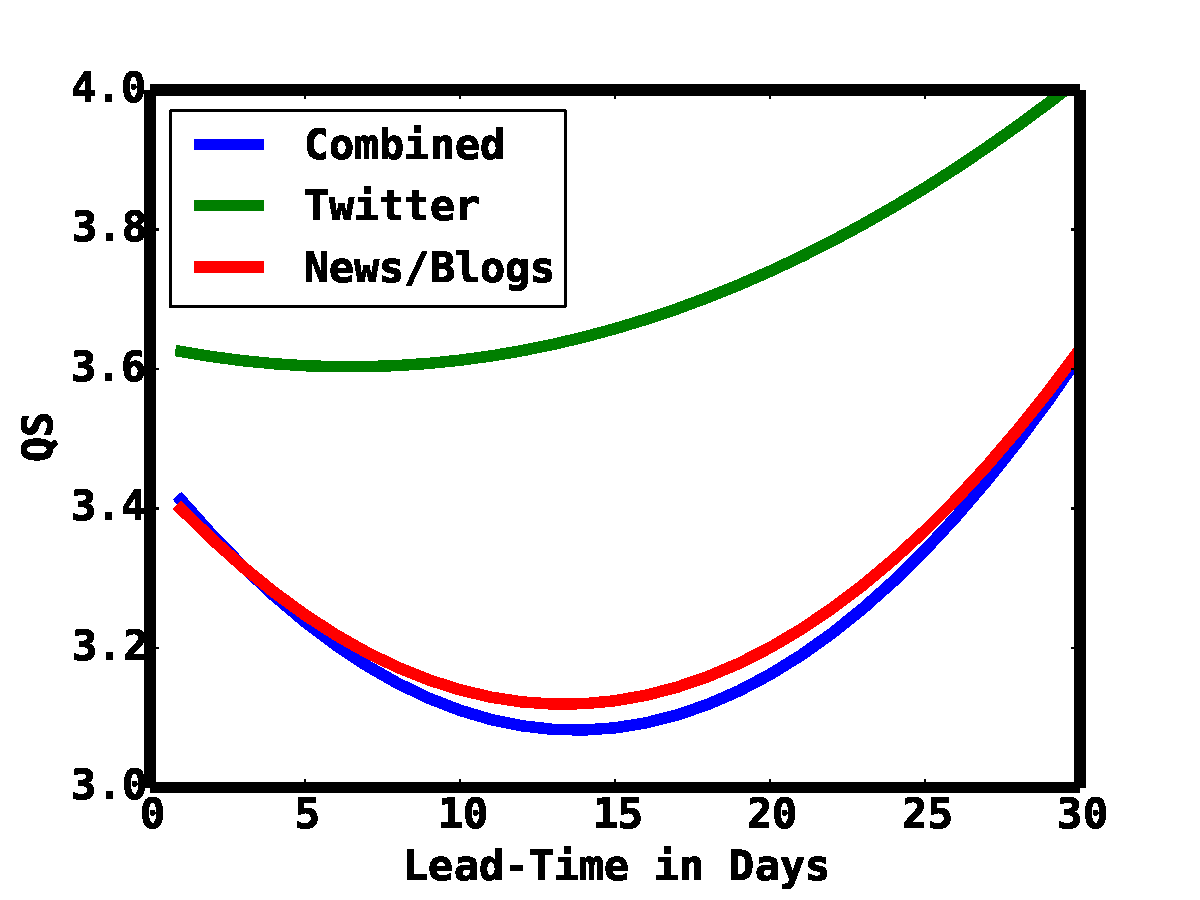
\includegraphics[scale=0.6]{leadTimeVsQS}
  \caption{Lead-Time vs Quality Score}
  \label{fig:leadTimeVsQS}
\end{figure*}

\noindent
{\bf What is the tradeoff between lead time and quality?}
Fig.~\ref{fig:leadTimeVsQS} shows that the QS of the planned protest model decreases (as expected) with lead time, initially, but
later rises again. The higher quality scores toward the right of Fig.~\ref{fig:leadTimeVsQS} are primarily due to
Facebook event pages.\\

\noindent
{\bf How does the method perform under stringent matching criteria?}
Fig.~\ref{fig:matchinginterval} shows the perfomance of the model when the matching window is varied from 7 to 1 in steps. 
We can see that the performance degrades quite gracefully even under the strict matching interval of a 1-day difference.\\

\begin{figure*}
  \centering
  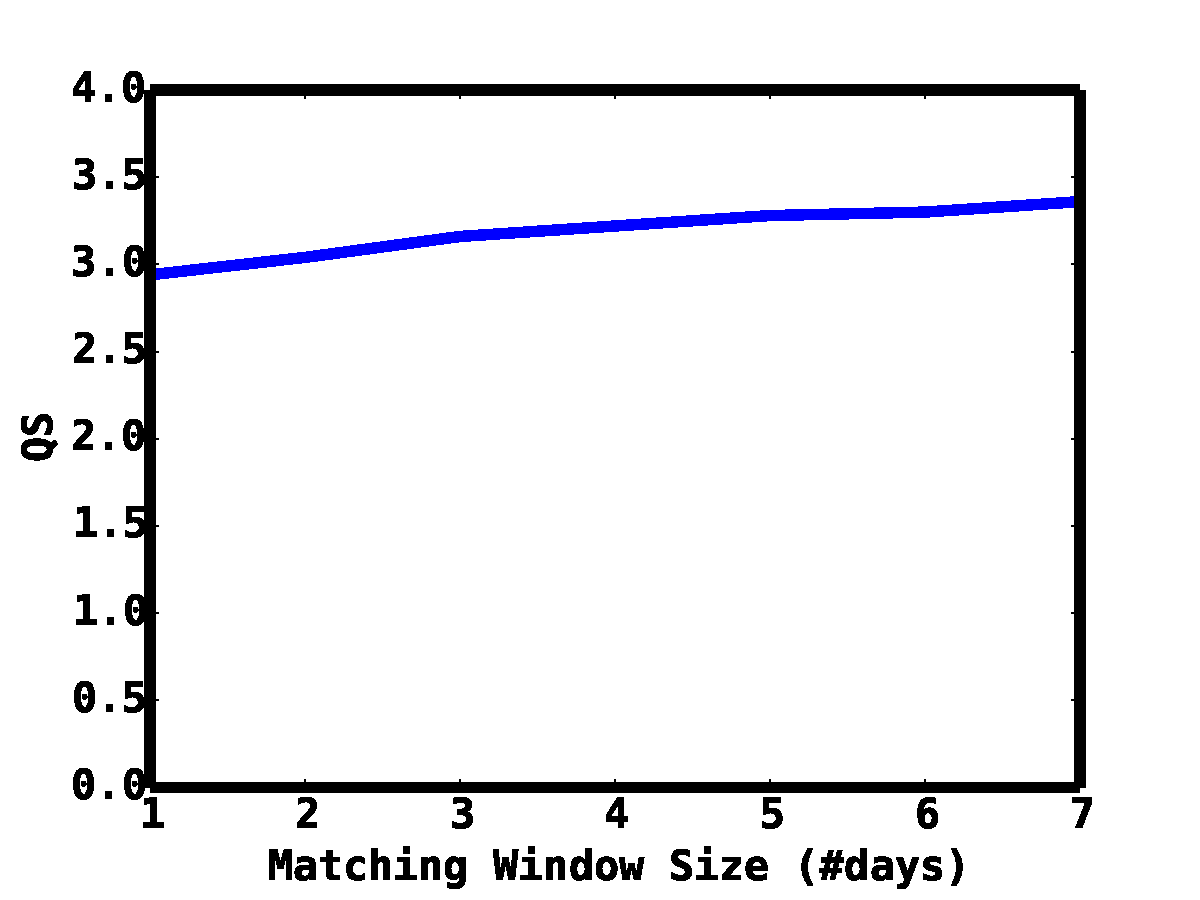
\includegraphics[scale=0.6]{matchingwindow}
  \caption{QS vs Matching Interval Trade-Off}
  \label{fig:matchinginterval}
\end{figure*}
\noindent
{\bf What is the distribution of quality scores?}
The clear mode toward the right side of the Fig.~\ref{fig:doubleHump} signifies that a majority of the planned 
protest alerts are of high quality. Further, the quality score distribution is unimodal suggesting that the careful
reasoning of locations and date normalization are crucial to achieving high quality.

\begin{figure*}
  \centering
  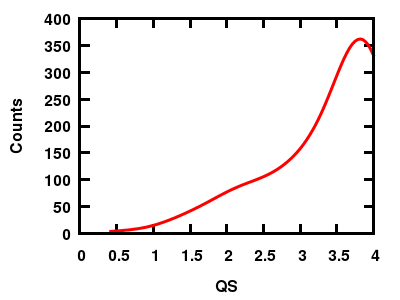
\includegraphics[scale=1]{doubleHump}
  \caption{Quality Score Distribution}
  \label{fig:doubleHump}
\end{figure*}

%\begin{subfigure}{\columnwidth}
%  \centering
%  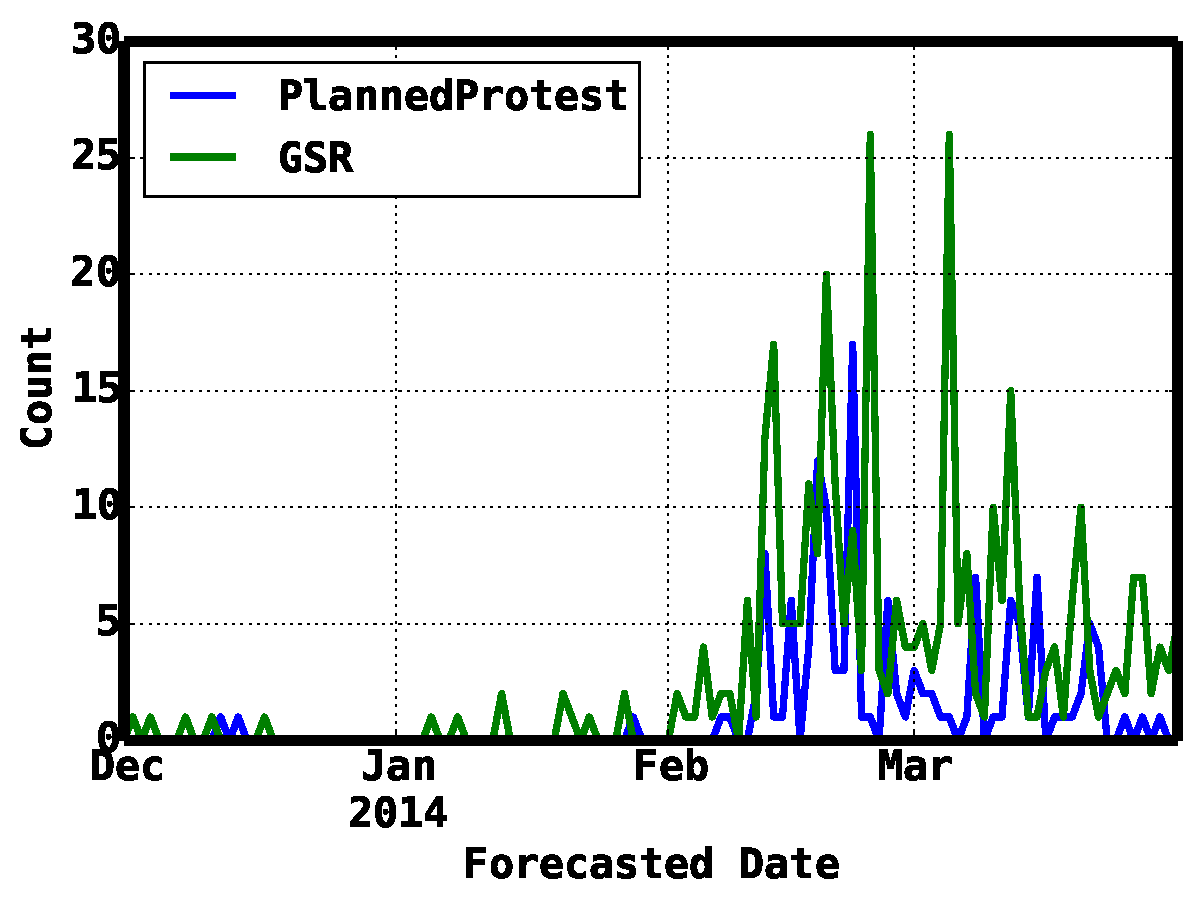
\includegraphics[width=\linewidth]{venezuela_violent}
%  \caption{Venezuelan Violent Protests}
%  \label{fig:venezuela_violent}
%\end{subfigure}%


%\begin{figure}
%    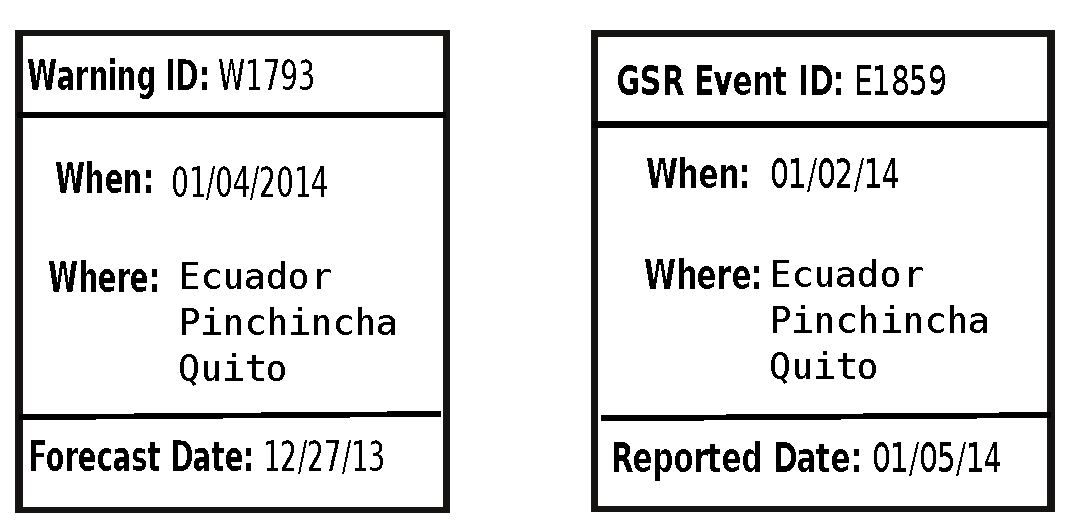
\includegraphics[width=0.5\textwidth]{alertstructure}
%    \caption{Structure of an Alert}
%    \label{fig:alertstructure}
%\end{figure}
%\begin{figure}
%    \includegraphics[width=0.5\textwidth]{timeline}
%    \caption{Matching Timeline}
%    \label{fig:timeline}
%\end{figure}


\chapter{Discussion}
\markright{Sathappan Muthiah \hfill Chapter 7. Discussion  \hfill}
We have described an approach to forecasting protests by detecting mentions of future events in news and social
media. The two twin issues of i) resolving the date and ii) resolving the location have been addressed satisfactorily
to realize an effective protest forecasting system. As different forms of communication media gain usage, systems
like ours will be crucial to understanding the concerns of citizenry.

Our future work is aimed at three aspects. First, to address situations such as nationwide protests and systems of protests,
we must generalize our system from generating protests at a single article level to digesting groups of articles. This will
require more sophisticated reasoning using PSL programs. 
Second, we would like to generalize our approach that currently
does detection of overt plans for protest to not-so-explicitly stated expressions of discontent. 
Finally, we plan to consider other population-level events of interest than just civil unrest, e.g., domestic political crises,
and design detectors to recognize the imminence of such events.



%%%%%%%%%%%%%%%%%%%%%%%%%%%%%%%%

% If you are using BibTeX, uncomment the following:
\cleardoublepage
%\phantomsection
\addcontentsline{toc}{chapter}{Bibliography}
\bibliographystyle{IEEEtran}
\markright{Sathappan Muthiah \hfill References \hfill}
\bibliography{references}

\end{document}
